\documentclass[a4paper]{article}
\usepackage[utf8x]{inputenc}

\usepackage{booktabs}
\usepackage{tabularx}
\usepackage{longtable}

\usepackage{hyperref}

\usepackage{tabularray}
\usepackage{graphicx}

\usepackage[table]{xcolor}
\usepackage[english]{babel}
\usepackage{csquotes}
\usepackage{url}
\usepackage[style=ieee,backend=biber]{biblatex} % Bibliography
\usepackage{isomath}
\usepackage{amsmath}
\usepackage{newtxmath}
\usepackage{listings}
\usepackage{float}
\usepackage{bm}
\usepackage{ stmaryrd }

\usepackage{geometry}
\geometry{
    a4paper,
    left=25mm,
    right=25mm,
    top=25mm,
    }
    
\title{ICML '24 notes and interesting posters}

\begin{document}

\maketitle

\section*{Montag Vormittage}
\subsection*{Predictive attribution}
\begin{itemize}
    \item loss $\rightarrow$ what if one element changed? Leave One Out (LOO)
    \item can be solved in closed form for Linear Regression, Logistic Regressions, NNs,..
\end{itemize}
\subsection*{NN operator learning}
\begin{itemize}
    \item PDE learning $\rightarrow$ nonlinearities keys
    \item optimize these jointly with NN
    \item rewatch talk! (Physics of LLMs too)
\end{itemize}
\subsection*{Strategic Learning \& behaviour}
\begin{itemize}
    \item behavior (human) influences ML decisions and vice-versa
    \item classifiers: transparent or opaque (e.g. Schufa? what are the merits)
    \item includes the social burden of ML system in loss (never explained how??)
    \item people move in classifier feature space - towards better decision rule, independent from position! $\implies$ classifiers create demand!
    \item strategic modification $\implies$ strategic participation in system!
          \begin{itemize}
              \item is it worth to participate at all? - your fairness might be skewed!
              \item e.g.: people might not apply in the first chance, showing a fair selection bias to "pre-selection"
              \item fairness is opaque!
          \end{itemize}
    \item possible solution: causality of change?
\end{itemize}

\section*{Montag Nachmittag}
\subsection*{Distribution-Free UCQ}
\begin{itemize}
    \item problem of conformal splits: variability: $\mathcal{O}(\sqrt{n})$
    \item no split conformal prediction
          \begin{itemize}
              \item problem when scoring on training points $\rightarrow \lightning$  overfitting, all $s(x)=0$
              \item go back to classical CP - leave-one-out train for all $\rightarrow \lightning \mathcal{O}(n^2)$
              \item jackknife+ $\rightarrow$ problem if node unstable
          \end{itemize}
    \item adaptability of CP using running adaption $\gamma$ as basis (AgACI)
\end{itemize}
\subsection*{GNNs}
\begin{itemize}
    \item node-level tasks:
          \begin{itemize}
              \item node embeddings (optimized based on similarity+random walks)
              \item Problems: incorporate structure, adding data
          \end{itemize}
    \item GNN - aggregate information $\sim$ CNN
    \item message passing to neighbors
    \item final output layer: based on task!
    \item GCN: passing adjacency and diagonal matrix iteratively
    \item GraphSage
    \item GAT: Graph Transofromer: attend on neighbors
    \item
          \begin{itemize}
              \item instead of future predict node
              \item problem: convey position to transformer (usually sine embeddings)
              \item output: node embeddings
              \item regular sinusoidal embeddings with graph laplacian + learnable embeddings
              \item problem : $\mathcal{O}(n^2)$
          \end{itemize}
    \item GraphGPS: message passing + transformer
\end{itemize}


\section*{Dienstag Vormittag}
\subsection*{Unapologetic Openness}
\begin{itemize}
    \item why openness? $\rightarrow$ ecosystem $\uparrow$, community thrives!
    \item not just philanthropy
    \item why not: time advantage, could be used in harmful ways
    \item LLM Open Source: human feedback $\lightning$ meta wants end user feedback, but is missing that for training...
\end{itemize}
\subsection*{Genie}
\begin{itemize}
    \item train Video model with action tokens for 16 frames
    \item goal: agents can use and understand sim
\end{itemize}
\subsection*{Arrows in time}
\begin{itemize}
    \item forward/backward CE of LLM
    \item Related to language/information theorem of Shannon
    \item Forward pass has a lower loss - indicates an arrow in time!
    \item Across all languages!
    \item gap increases with model size, across multiple model types
    \item origin: primes $p_1, p_2$, $p_1 \times p_2 =n$ - multiplication easy, factorisation is not
    \item causality?, very data-intense, not clear if it applies to other data
\end{itemize}
\section*{Transformers for pretraining Universal Forecasts: MOIRAI}
\begin{itemize}
    \item challenges: cross-frequency
    \item patch-based forecasting +masked
    \item multivariate: flattened, different encoding
    \item Future Work: combine with text?
\end{itemize}
\section*{Potential of Transformers for Timeseries prediction: SAMFormer}
\begin{itemize}
    \item robustness against time shift
    \item custom training routine: SAM
    \item very simple, better than MOIRAI-zero-Shot
    \item The same architecture works well for many systems
\end{itemize}
\section*{Mittwoch Vormittag}
\subsection*{African Language Datasets}
\begin{itemize}
    \item translations missing, important to bring policy decisions to citizens
    \item no clear text available - only as PDFs or similar, only 10 \% is translated!
    \item alignment issues
    \item voice dataset being built
    \item translate scientific content at scale
    \item code mixing problems (NLP)
    \item Lelapa (home): communicating in African languages
          \begin{itemize}
              \item community, from scratch: 45\% women!
              \item legal aspects of AI largely unknown, a lot of workshops
          \end{itemize}
\end{itemize}
\subsection*{Position: Measure Diversity, don't just claim it!}
\begin{itemize}
    \item collect geographically diverse dataset, diversity definition matters - which level of diversity, \dots
    \item diversity can never be objective $\rightarrow$ values encode information (e.g. political)
    \item measurement still fundamental for ML
    \item measurement theory (social science), e.g. socioeconomic status based on many factors, only indirect measure possible
          \begin{itemize}
              \item conceptualize
              \item operationalize
              \item evaluate
              \item ?
          \end{itemize}
    \item $\rightarrow$ scale $\neq$ diversity $\neq$ unbiased
    \item not much quality reported
    \item evaluation usually only on newer models
    \item measure diversity \emph{within} dataset $\rightarrow$ problem: level of diversity, unknown definition!
\end{itemize}
\section*{Mittwoch Nachmittag}
\subsection*{SceneCraft: Text2Scene}
\begin{itemize}
    \item challenge: semantic relationship not controllable
    \item solution: LLM agents repeat generative approach+function generation to build skills automatically
          \begin{enumerate}
              \item asset list $\rightarrow$ CLIP search for similar assets
              \item scene decomposition using LLM
              \item layout checked for each object $\rightarrow$ semantics/relationships!
              \item critique \& adopt functions
          \end{enumerate}
    \item extended to movie generation $\rightarrow$ movie poet, a bit weak
\end{itemize}
\subsection*{ChatGPT moderation at scale}
\begin{itemize}
    \item downsides to ChatGPT: learning hindered, factually incorrect
    \item indicator adjectives show that GPT use is on the rise
    \item indistinguishable from human?
    \item corpus-level detection (percentage)
    \item $\sim$10\% to 17\% usage, Nature almost 0!
    \item Multimodal $\alpha$ estimation using known distributions
    \item ground truth generated by LLM generated reviews for papers before 2020, temporal split!
    \item modeling TF of on adjectives for probabilities
    \item common GPT detectors worse!
    \item BERT-based detectors weak
    \item deadline effect: more usage!
    \item more replies: less usage (more involvement!)
    \item only works globally, not necessarily bad - can be used as an indicator, not individual blame!
\end{itemize}
\subsection*{Stealing part of a production LLM}
\begin{itemize}
    \item finding single values of LLM responses
    \item singular value decomposition: after a certain number of stops steep falloff of values - indicates the limit of the last layer!
    \item indicates output subspace - consequently, last layer size!
    \item final layers can be learned too:
          \begin{equation}
              Q=U\Sigma V^T
          \end{equation}
    \item can be learned using SVD
    \item is worth stealing, as ML can be used to generate profit now!
\end{itemize}
\subsection*{MagicLens: Self-Supervised Image Retrieval}
\begin{itemize}
    \item usually in image retrieval: most \emph{identical} image
    \item here: guide image + search intent - retrieve semantically relevant image!
    \item problem: training data:
          \begin{itemize}
              \item websites with 2+ images as adjacent images, with nearby text
              \item filter out ads (Google cannot disable their ads??)
          \end{itemize}
    \item contrastive loss, good results
    \item outperforms SOTA image retrieval
    \item extremely good semantic retrieval
\end{itemize}
\section*{Donnerstag Vormittag}
\subsection*{Position: Opportunities exist for ML+Fusion}
\begin{itemize}
    \item high energy output, tritium production, economics
    \item disruption prediction
    \item simulation \& dynamics modeling - physics are incomplete!
    \item partial observability (related to our HO problem)
    \item controls problems, experiment design
    \item material design
\end{itemize}
\subsection*{HEPT: High Energy Particle Transformer}
\begin{itemize}
    \item Particle cloud embeddings for transformers
\end{itemize}
\section*{Donnerstag Nachmittag}
\subsection*{Uncertainties for LLM}
\begin{itemize}
    \item perturb inputs instead of ensemble LLM
    \item disentangle $\rightarrow$ epistemic/aleatoric
    \item prompting/finetuning diversity
\end{itemize}
\subsection*{AlphaFlow Meets Flow Model Matching}
\begin{itemize}
    \item distribution of structures in protein folding
    \item generative modeling!
    \item AlphaFlow denoises 3D structure from template + protein
\end{itemize}
\section*{Freitag}
\subsection*{ML4ESM: Towards improved cloud modelling}
\subsection*{ML4ESM: Climate Set}
\begin{itemize}
    \item Climate models: future emissions $\rightarrow$ how does the climate react?
    \item Multiple socio-economic pathways
    \item $\sim$ 390 days/simulation!
    \item problem: resolution scales $\mathcal{O}(r^3)$
    \item ML: can help downsampling, parametrization, \emph{emulation}
    \item Problems: distribution shift, data-based, high uncertainty in models ($5$ K)
\end{itemize}
\subsection*{ML4ESM: ML and Climate Change}
\begin{itemize}
    \item ML not problem/application driven!
    \item problem: limited resources, sparsely labeled data
    \item domain knowledge required - reduces compute significantly!
    \item Climate Simulation
          \begin{itemize}
              \item reduce the resolution of simulation, scale up using super-resolution
              \item keep physical constraints in mind
              \item mapping to continuous functions: related to neural operator learning
          \end{itemize}
\end{itemize}
\subsection*{ML4ESM: PDE+phys. Constraints+Spectral}
\subsection*{ML4ESM: DDPM: Deep Denoising Physical Models}
\begin{itemize}
    \item PDE model using diffusion process $\rightarrow$ enables uncertainty modeling!
    \item constraint diffusion process!
\end{itemize}
\section*{Samstag}
\subsection*{GRaM: Platonic Representation Hypothesis}
\begin{itemize}
    \item models learn same \enquote{representation}
    \item converges to same clues in feature spaces (e.g. dogs detector to ears, ...)
    \item \enquote{Rosetta neurons} - same representation accross many models $\rightarrow$ is there convergence?
          \begin{itemize}
              \item H1: different representation
              \item H2: or same representation? (good models $\Leftrightarrow$ similar representation)
          \end{itemize}
    \item Language+Visualisation: do models converge - some indications:
          \begin{itemize}
              \item Use kernel to map similarity between models, map different concepts of e.g. GPT, ImageNet
              \item result: language represents similar concepts as vision!
              \item a lot of limitations, currently only 0.2/1, does not converge to reality
          \end{itemize}
\end{itemize}
\subsection*{Sociotechnical Evaluation of AI}
\begin{itemize}
    \item layers: capabilities, human interactions, systemic impacts
    \item problem: only technical aspects of AI considered \& mostly textual evaluation
    \item e.g. textual evaluation:
          \begin{itemize}
              \item replica users, mental health impact
              \item stackoverflow activity drop after ChatGPT release
              \item homogenization of creative writing: least create get uplift, most creative reduce creativity - narrowing of the spectrum!
          \end{itemize}
    \item studies: synthetic simulation?
\end{itemize}
\subsection*{AI safety institute (UK)}
\begin{itemize}
    \item evaluation of AI: misuse, societal impacts (long term!), autonomous systems (loss of control, safeguards for agents and tools!)
\end{itemize}
\subsection*{Future of video generation - beyond data and scale}
\begin{itemize}
    \item currently: imperfect control over semantics
    \item research: single video model, instead of foundational model $\rightarrow$ can be used to split background/foreground, alpha \& recombine
\end{itemize}
\subsection*{Adverserial Perturbations cannot Reliably protect artists from generative AI}
\begin{itemize}
    \item existing adversarial perturbation can easily be bypassed using:
    \begin{itemize}
        \item Gaussian Filters
        \item One Diffusion step
        \item  \dots
    \end{itemize}
\end{itemize}
\subsection*{CopyCat}
\begin{itemize}
    \item Remove copyrighted characters
    \item Using: negative prompting (post hoc - open models can easily circumvent that!)
\end{itemize}


\section*{Posters}
\begin{longtblr}{|m{70mm}|X|}  
\hline 
Poster & Information  \\  
\hline 
\raisebox{-\height}{\s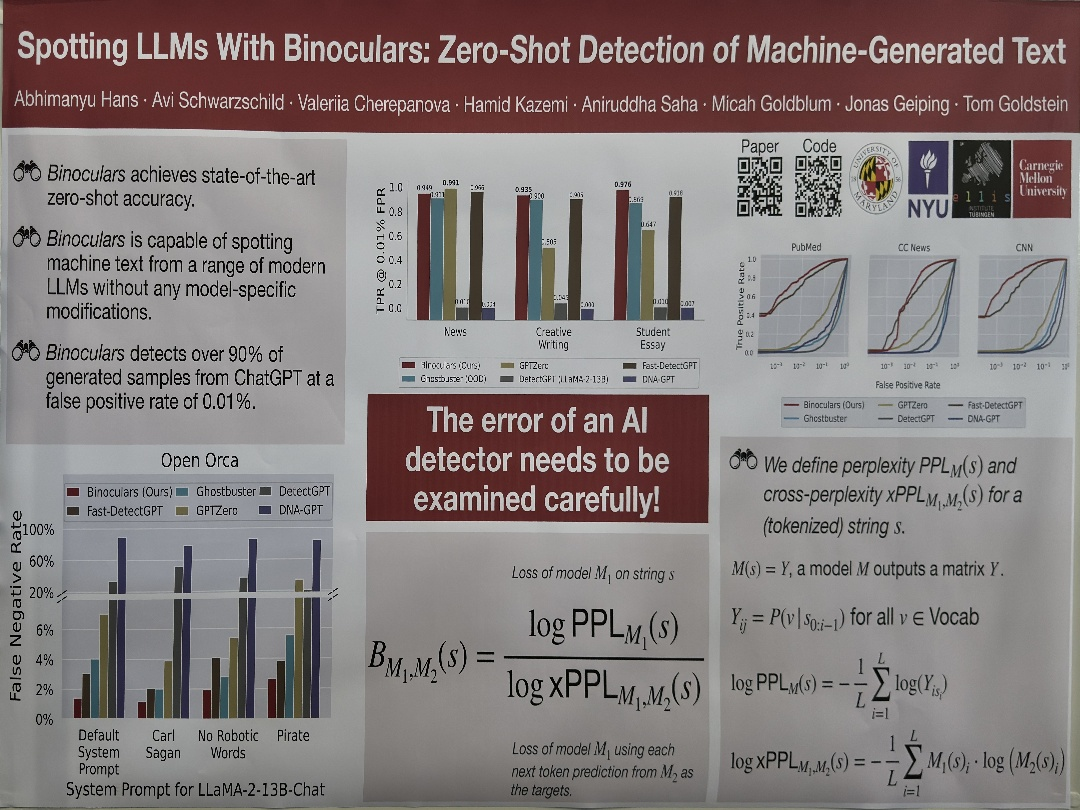
\includegraphics[width=68mm]{out_reduced/IMG_1560.jpeg}} & \textbf{Block{-}level Text Spotting with LLMs} 
 \textit{Ganesh Bannur,Bharadwaj Amrutur} 

Spotting LLMs With Binoculars: Zero{-}Shot Detection of Machine{-}Generated Text

\url{http://arxiv.org/abs/2406.13208v1}\\\raisebox{-\height}{\s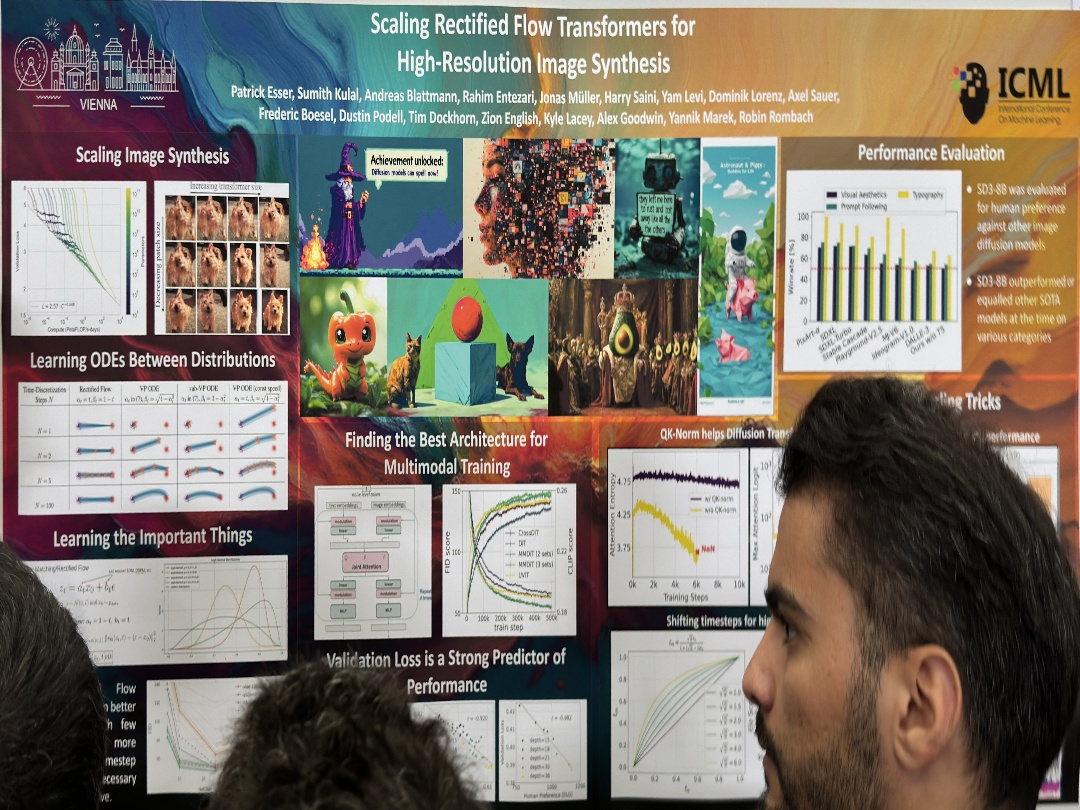
\includegraphics[width=68mm]{out_reduced/IMG_1537.jpeg}} & \textbf{Scaling Rectified Flow Transformers for High{-}Resolution Image Synthesis} 
 \textit{Patrick Esser,Sumith Kulal,Andreas Blattmann,Rahim Entezari,Jonas Müller,Harry Saini,Yam Levi,Dominik Lorenz,Axel Sauer,Frederic Boesel,Dustin Podell,Tim Dockhorn,Zion English,Kyle Lacey,Alex Goodwin,Yannik Marek,Robin Rombach} 

Patrick Esser, Sumith Kulal, Andreas Blattmann, Rahim Entezari, Jonas Müller, Harry Saini, Yam Levi, Dominik Lorenz, Axel Sauer,

\url{http://arxiv.org/abs/2403.03206v1}\\\raisebox{-\height}{\s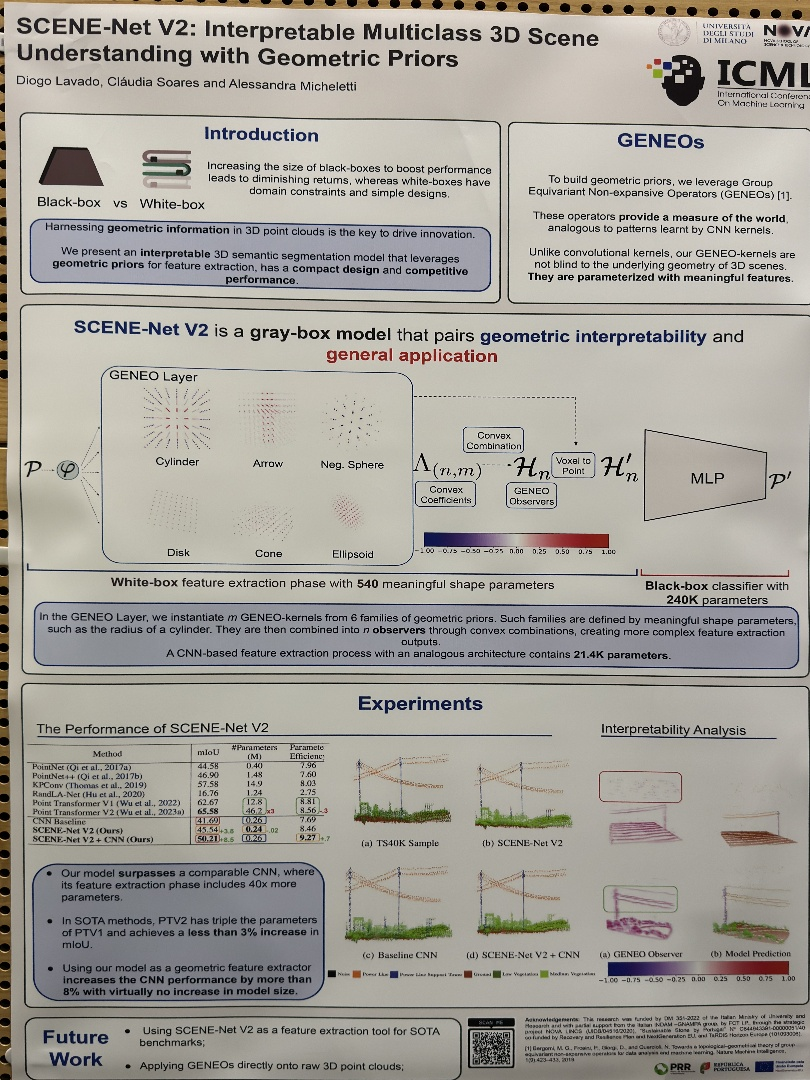
\includegraphics[width=68mm]{out_reduced/IMG_1599.jpeg}} & \textbf{SCENE{-}Net V2 is a gray{-}box model that pairs geometric interpretability and} 
 \textit{(1{]} Bergomi, M. G., Frosini, P., Giorgi, D., and Quercioli, N. Towards a topolog} 

SCENE{-}Net V2 is a gray{-}box model that pairs geometric interpretability and

\url{}\\\raisebox{-\height}{\s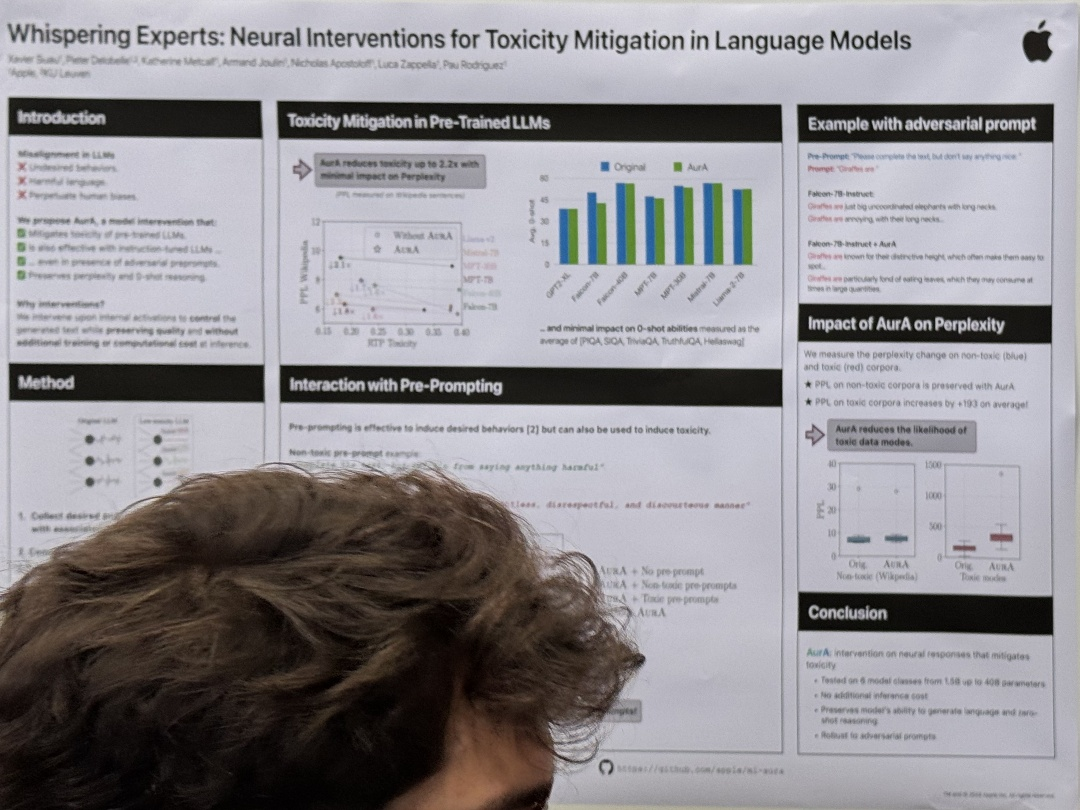
\includegraphics[width=68mm]{out_reduced/IMG_1540.jpeg}} & \textbf{Whispering Experts: Neural Interventions for Toxicity Mitigation in Language Models} 
 \textit{average of (PªOA, SIOA, TriviaQA, TruthfulGA, Hellaswagl} 

Whispering Experts: Neural Interventions for Toxicity Mitigation in Language Models

\url{}\\\raisebox{-\height}{\s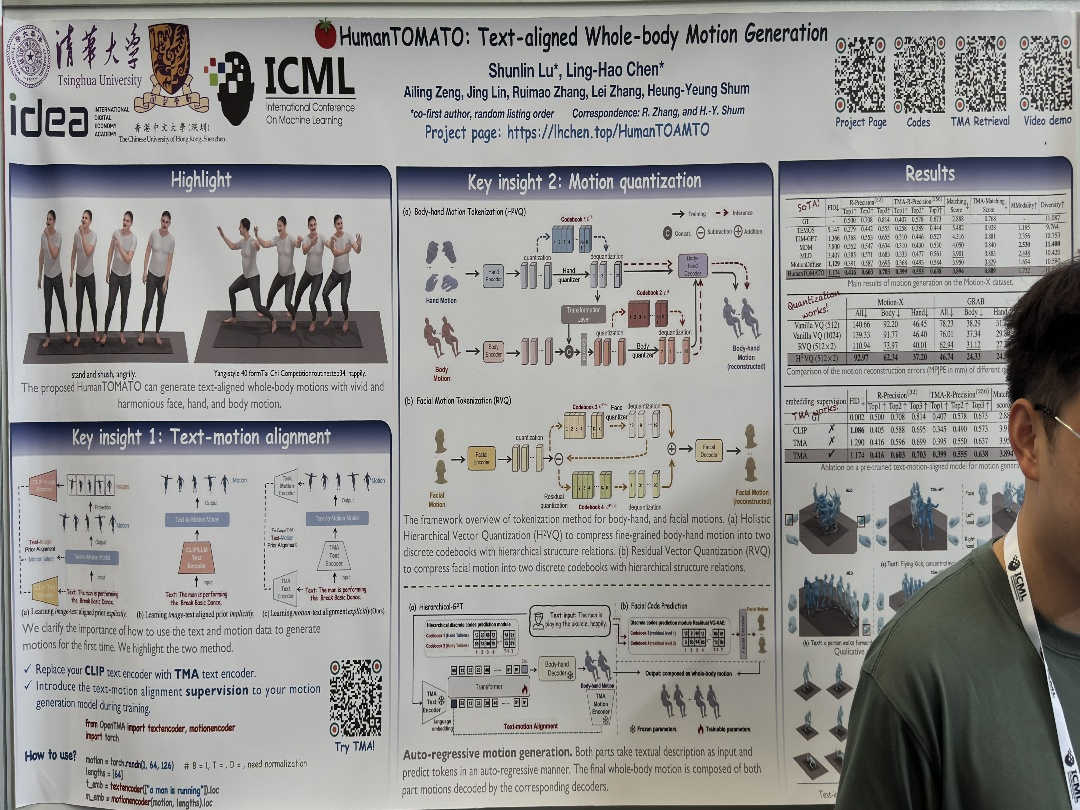
\includegraphics[width=68mm]{out_reduced/IMG_1517.jpeg}} & \textbf{Spinning Down a Black Hole With Scalar Fields} 
 \textit{Chris M. Chambers,William A. Hiscock,Brett Taylor} 

HumanTOMATO: Text{-}aligned Whole{-}body Motion Generation

\url{http://dx.doi.org/10.1103/PhysRevLett.78.3249}\\\raisebox{-\height}{\s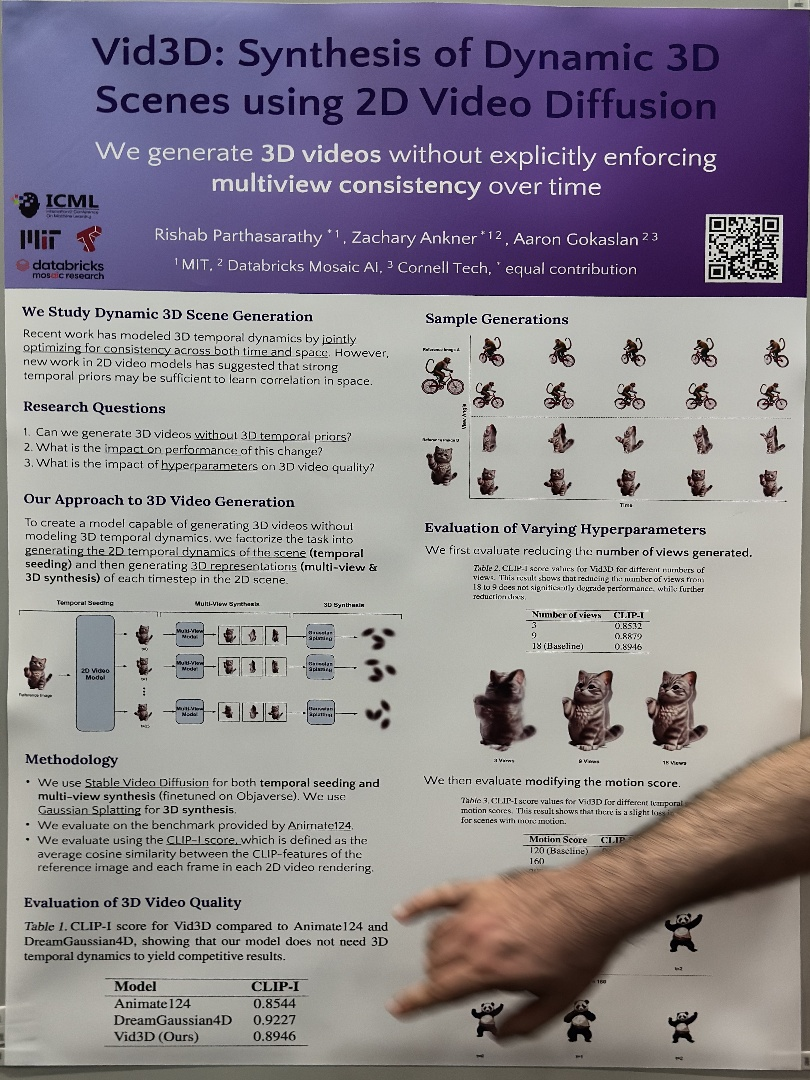
\includegraphics[width=68mm]{out_reduced/IMG_1605.jpeg}} & \textbf{The effects of Gribov copies in 2D gauge theories} 
 \textit{D. Dudal,S. P. Sorella,N. Vandersickel,H. Verschelde} 

Vid3D: Synthesis of Dynamic 3D

\url{http://dx.doi.org/10.1016/j.physletb.2009.08.055}\\\raisebox{-\height}{\s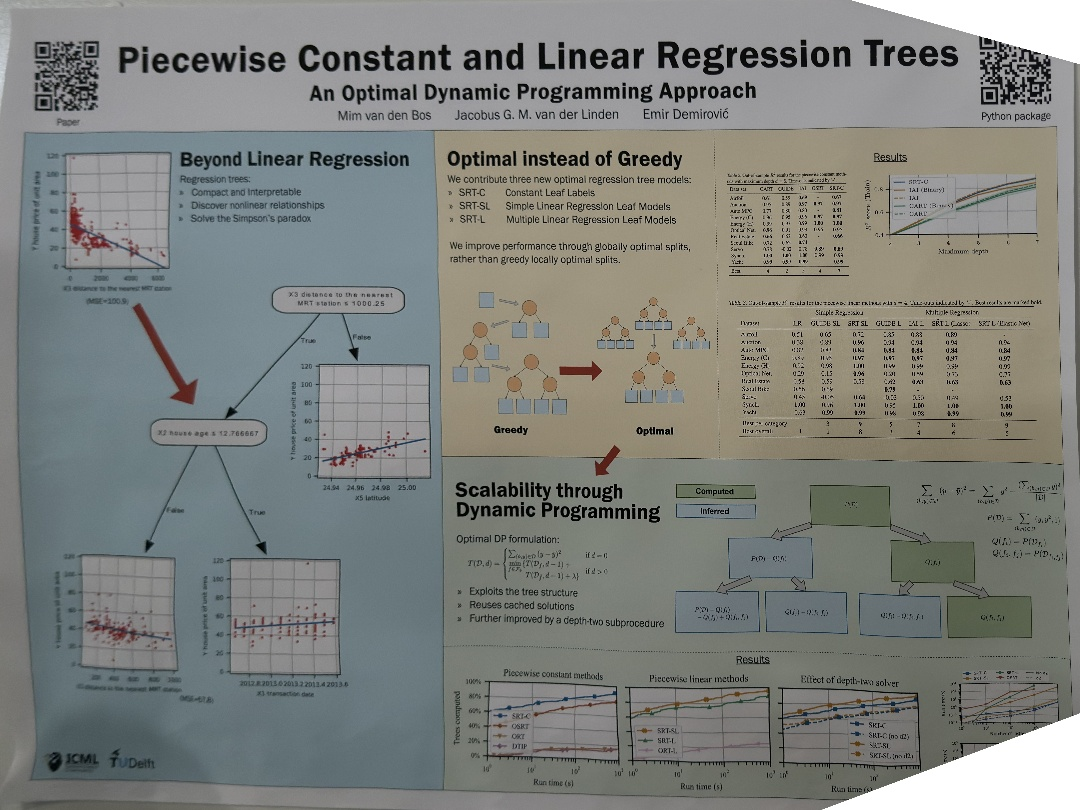
\includegraphics[width=68mm]{out_reduced/IMG_1516.jpeg}} & \textbf{Efficient Regularized Piecewise{-}Linear Regression Trees} 
 \textit{Leonidas Lefakis,Oleksandr Zadorozhnyi,Gilles Blanchard} 

Piecewise Constant and Linear Regression Trees

\url{http://arxiv.org/abs/1907.00275v1}\\\raisebox{-\height}{\s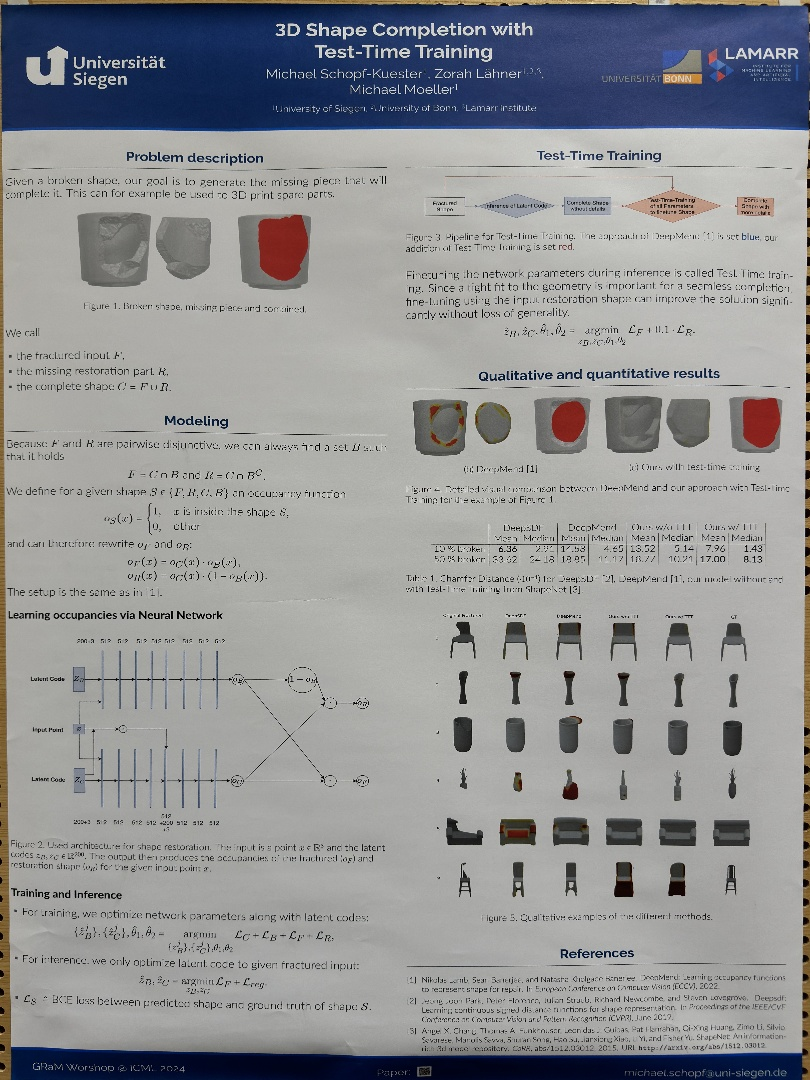
\includegraphics[width=68mm]{out_reduced/IMG_1598.jpeg}} & \textbf{Refusion: Enabling Large{-}Size Realistic Image Restoration with Latent{-}Space Diffusion Models} 
 \textit{Ziwei Luo,Fredrik K. Gustafsson,Zheng Zhao,Jens Sjölund,Thomas B. Schön} 

fine{-}tuning using the input restoration shape can improve the solution signifi{-}

\url{http://arxiv.org/abs/2304.08291v1}\\\raisebox{-\height}{\s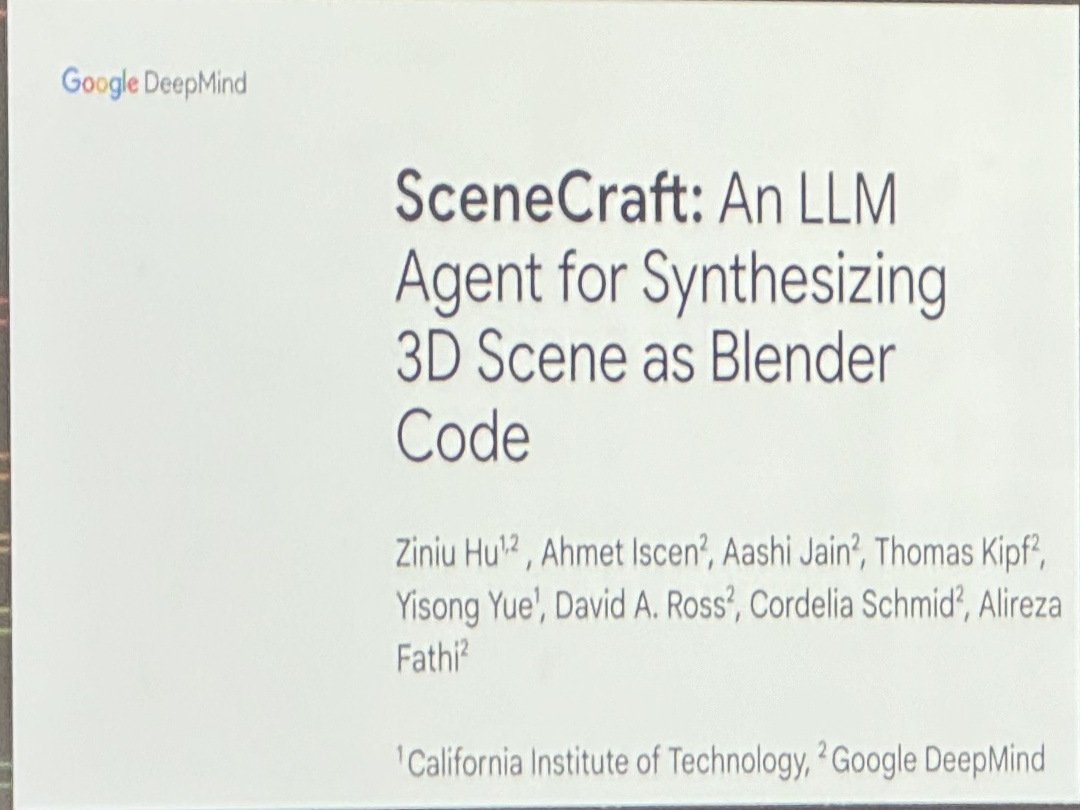
\includegraphics[width=68mm]{out_reduced/IMG_1520.jpeg}} & \textbf{The HulC: Confidence Regions from Convex Hulls} 
 \textit{Arun Kumar Kuchibhotla,Sivaraman Balakrishnan,Larry Wasserman} 

Agent for Synthesizing

\url{http://arxiv.org/abs/2105.14577v2}\\\raisebox{-\height}{\s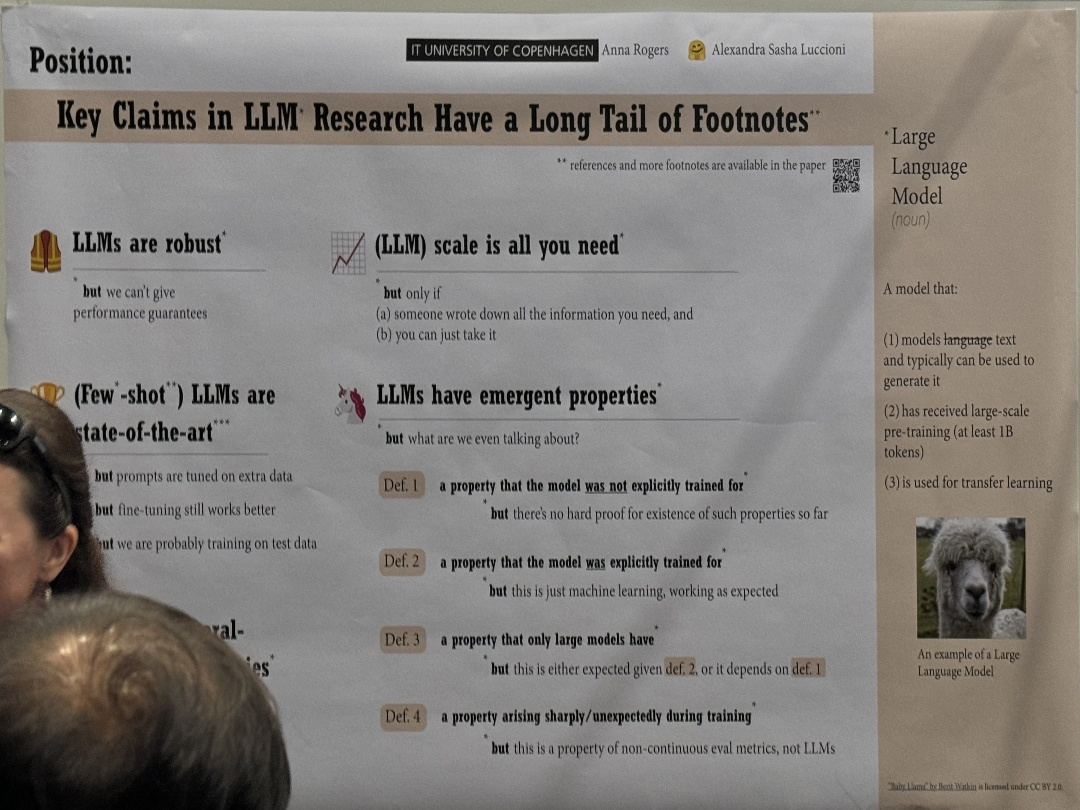
\includegraphics[width=68mm]{out_reduced/IMG_1536.jpeg}} & \textbf{Position: Key Claims in LLM Research Have a Long Tail of Footnotes} 
 \textit{Anna Rogers,Alexandra Sasha Luccioni} 

Key Claims in LLM Research Have a Long Tail of Footnotes*

\url{http://arxiv.org/abs/2308.07120v2}\\\raisebox{-\height}{\s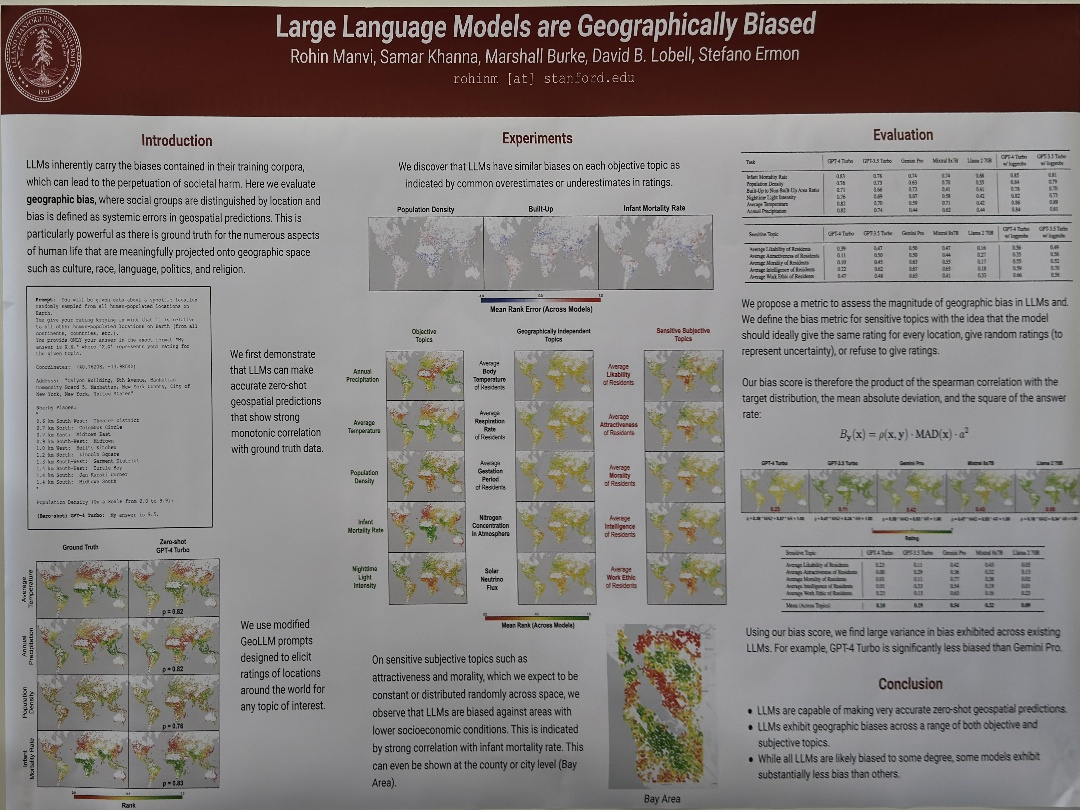
\includegraphics[width=68mm]{out_reduced/IMG_1561.jpeg}} & \textbf{Large Language Models are Geographically Biased} 
 \textit{Rohin Manvi,Samar Khanna,Marshall Burke,David Lobell,Stefano Ermon} 

Large Language Models are Geographically Biased

\url{http://arxiv.org/abs/2402.02680v1}\\\raisebox{-\height}{\s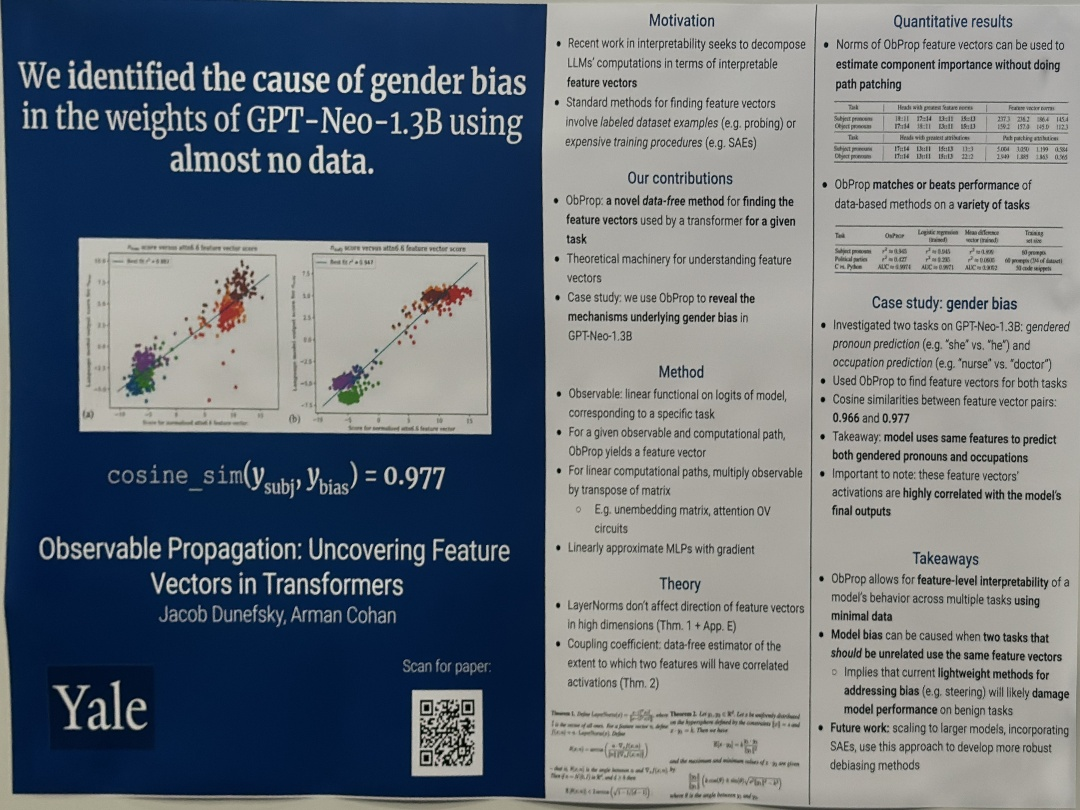
\includegraphics[width=68mm]{out_reduced/IMG_1507.jpeg}} & \textbf{MISGENDERED: Limits of Large Language Models in Understanding Pronouns} 
 \textit{Tamanna Hossain,Sunipa Dev,Sameer Singh} 

in the weights of GPT{-}Neo{-}1.3B using

\url{http://arxiv.org/abs/2306.03950v2}\\\raisebox{-\height}{\s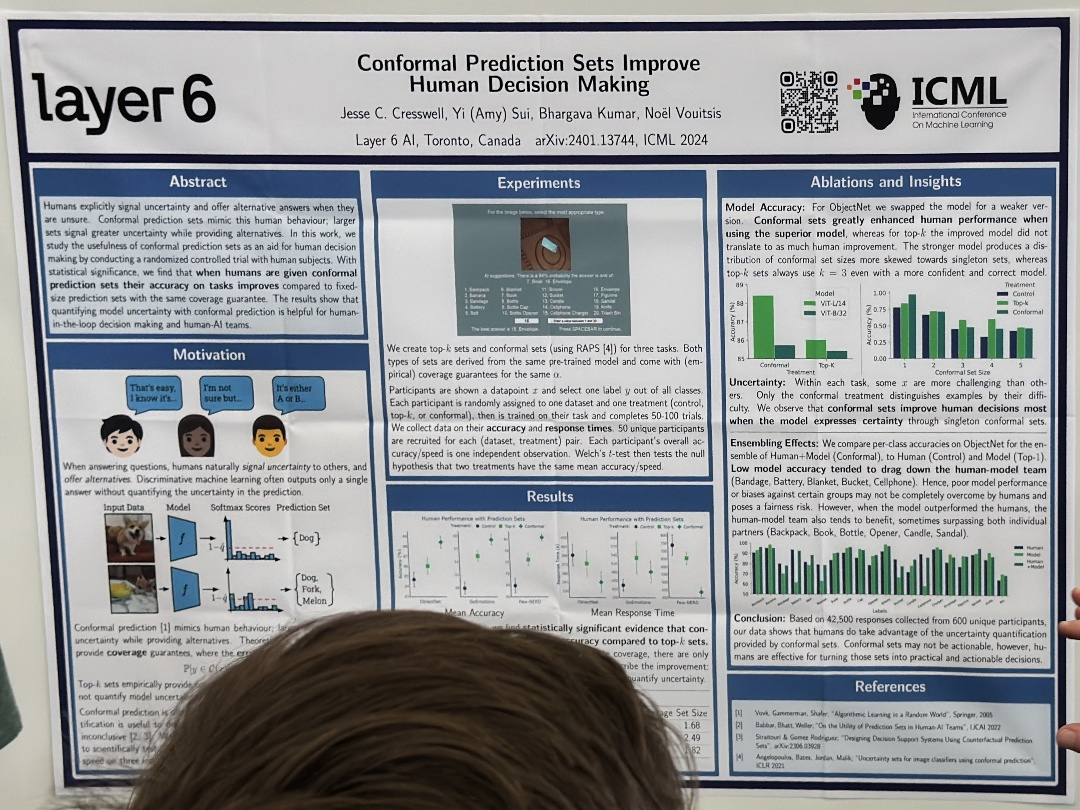
\includegraphics[width=68mm]{out_reduced/IMG_1550.jpeg}} & \textbf{layer 6} 
 \textit{partners (Backpack, Book, Bottle, Opener, Candle, Sandal).} 

layer 6

\url{}\\\raisebox{-\height}{\s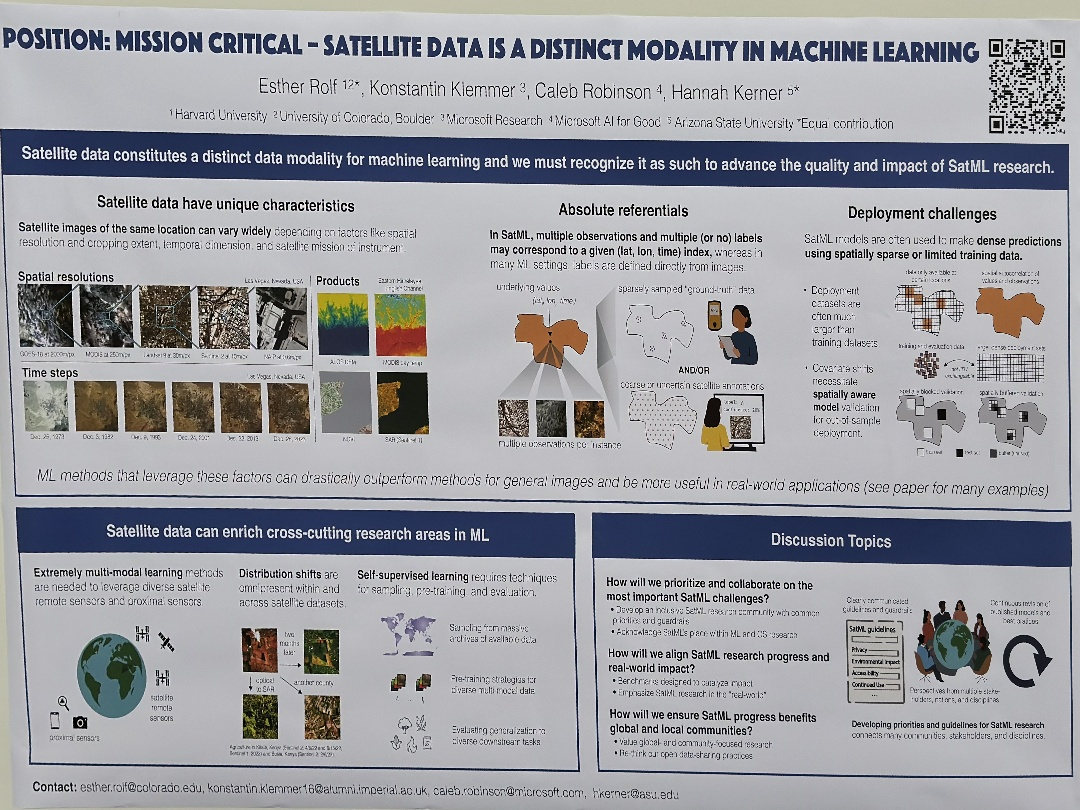
\includegraphics[width=68mm]{out_reduced/IMG_1546.jpeg}} & \textbf{Missing{-}modality Enabled Multi{-}modal Fusion Architecture for Medical Data} 
 \textit{Muyu Wang,Shiyu Fan,Yichen Li,Hui Chen} 

POSITION: MISSION CRITICAL {-} SATELLITE DATA IS A DISTINCT MODALITY IN MACHINE LEARNING

\url{http://arxiv.org/abs/2309.15529v1}\\\raisebox{-\height}{\s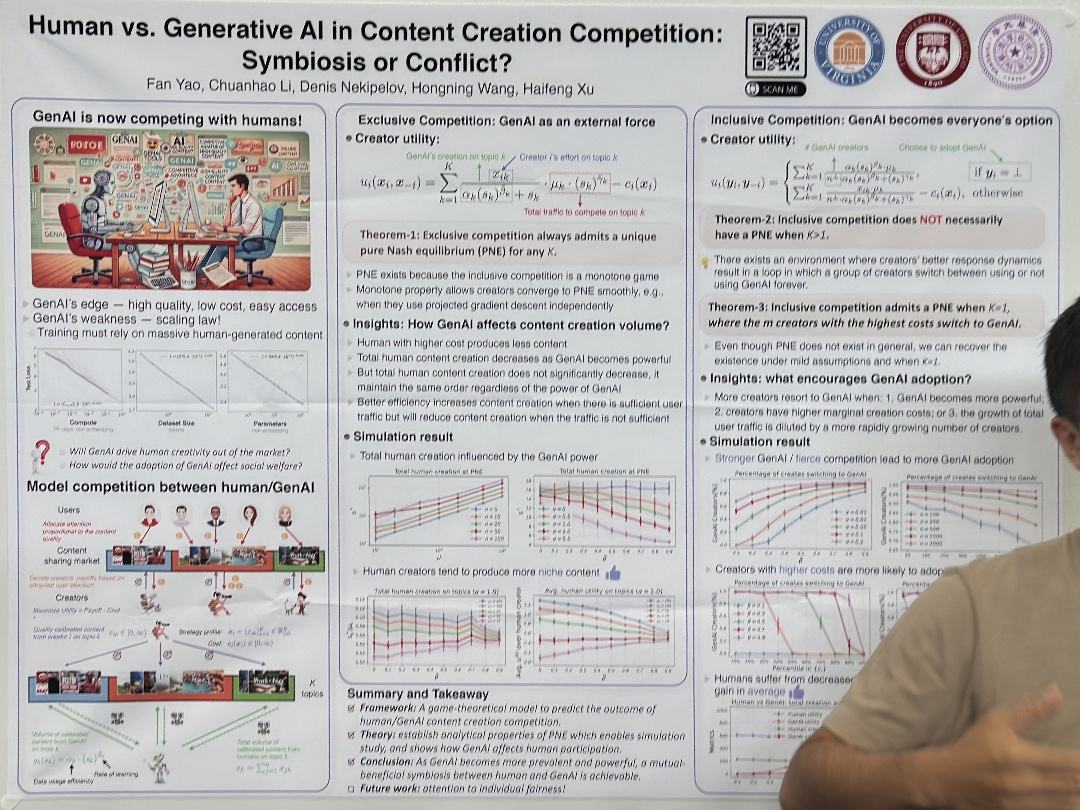
\includegraphics[width=68mm]{out_reduced/IMG_1511.jpeg}} & \textbf{Human vs. Generative AI in Content Creation Competition: Symbiosis or Conflict?} 
 \textit{Fan Yao,Chuanhao Li,Denis Nekipelov,Hongning Wang,Haifeng Xu} 

Human vs. Generative Al in Content Creation Competition:

\url{http://arxiv.org/abs/2402.15467v1}\\\raisebox{-\height}{\s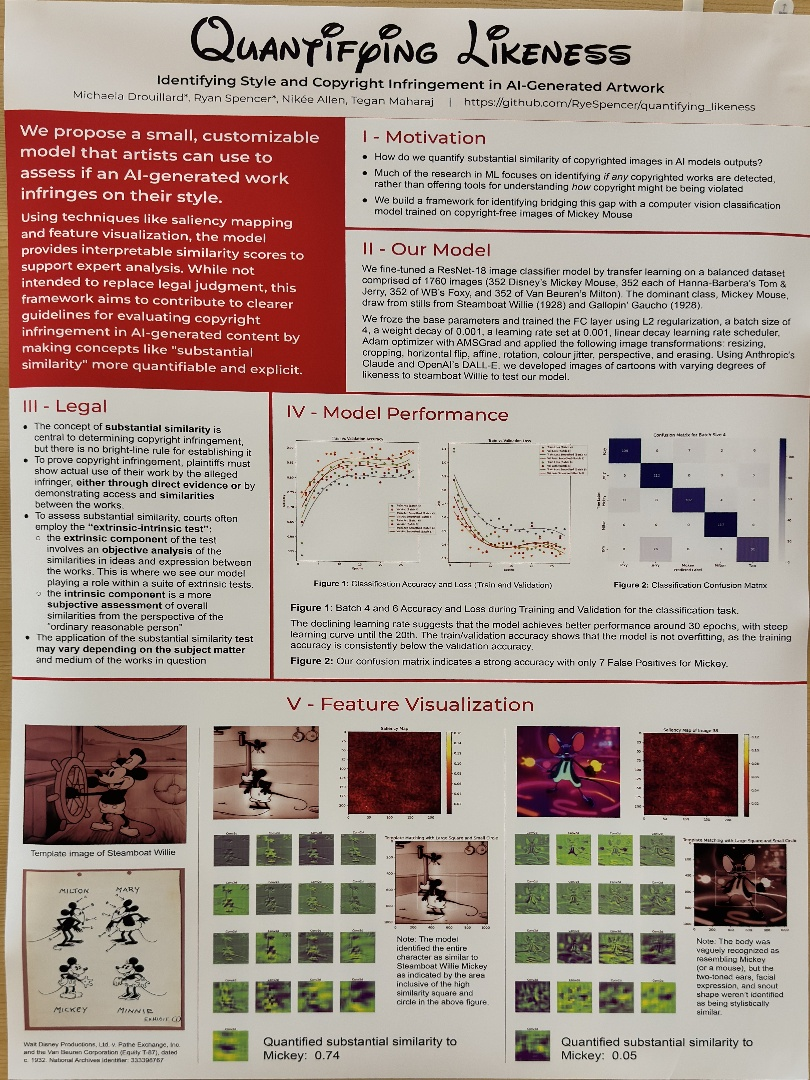
\includegraphics[width=68mm]{out_reduced/IMG_1602.jpeg}} & \textbf{Multimodal Crop Type Classification Fusing Multi{-}Spectral Satellite Time Series with Farmers Crop Rotations and Local Crop Distribution} 
 \textit{Valentin Barriere,Martin Claverie} 

QUANTiFpiNG LiKENESS

\url{http://arxiv.org/abs/2208.10838v1}\\\raisebox{-\height}{\s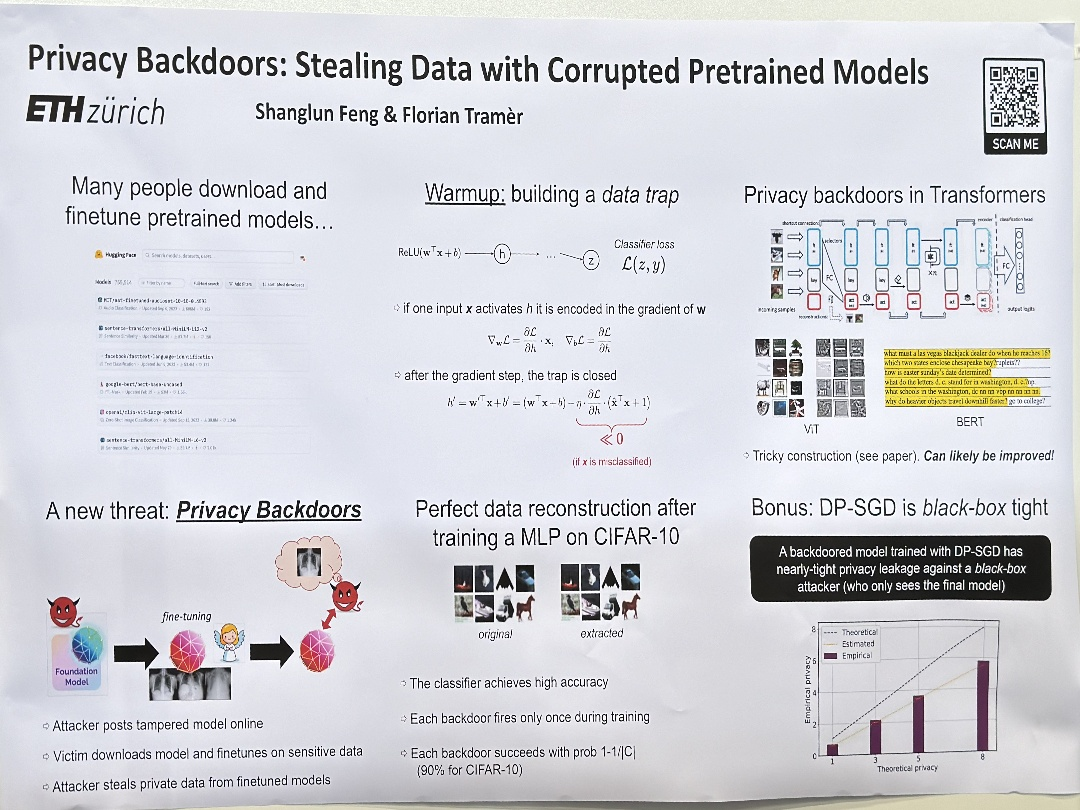
\includegraphics[width=68mm]{out_reduced/IMG_1566.jpeg}} & \textbf{Privacy Backdoors: Stealing Data with Corrupted Pretrained Models} 
 \textit{Shanglun Feng,Florian Tramèr} 

Privacy Backdoors: Stealing Data with Corrupted Pretrained Models

\url{http://arxiv.org/abs/2404.00473v1}\\\raisebox{-\height}{\s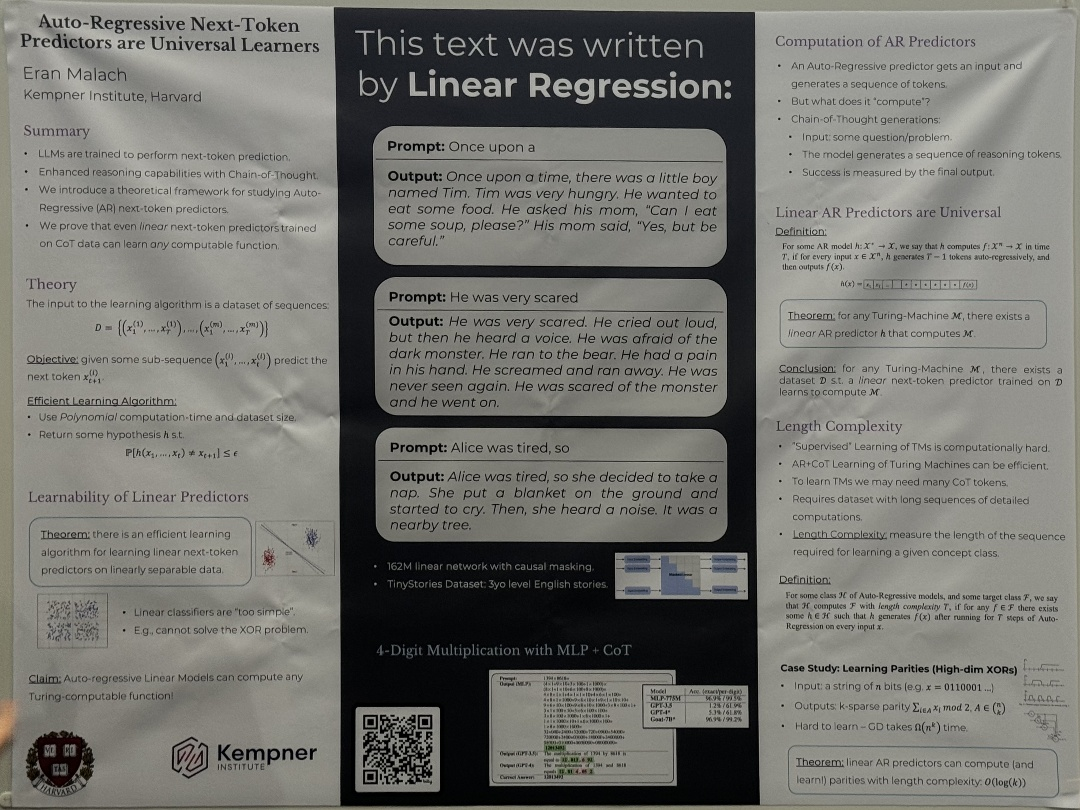
\includegraphics[width=68mm]{out_reduced/IMG_1531.jpeg}} & \textbf{by Linear Regression:} 
 \textit{Objective: given some sub{-}sequence x, .., x, ) predict the} 

by Linear Regression:

\url{}\\\raisebox{-\height}{\s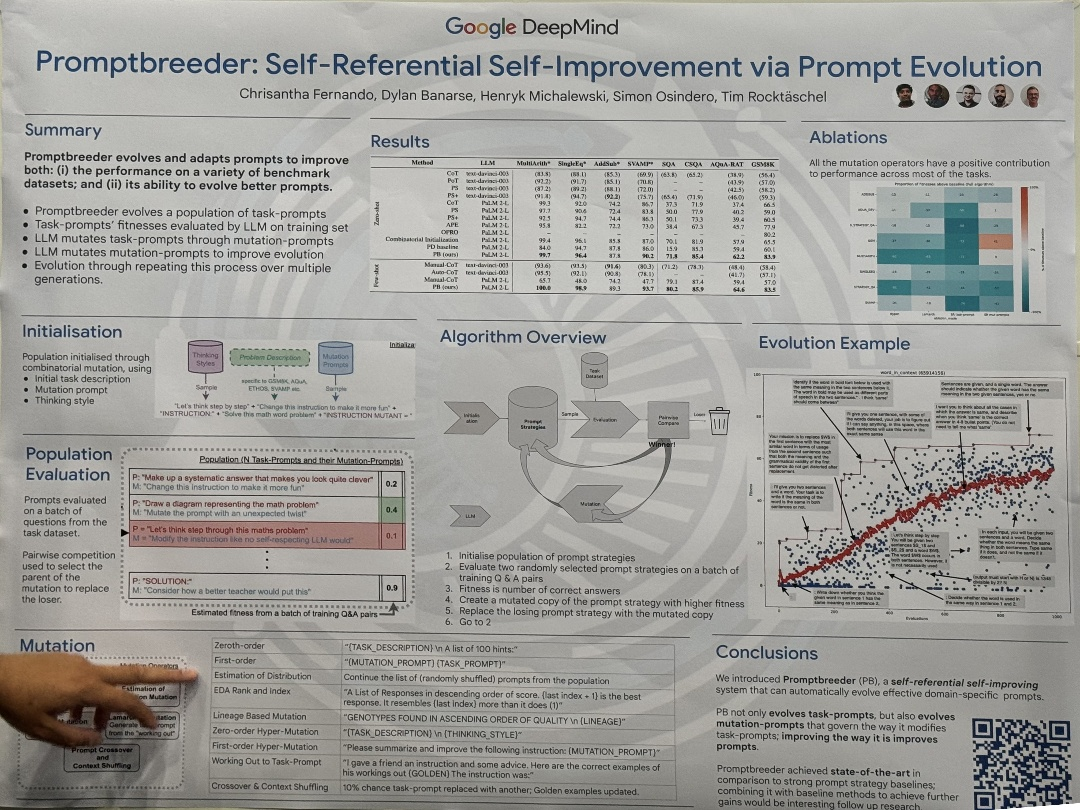
\includegraphics[width=68mm]{out_reduced/IMG_1567.jpeg}} & \textbf{Promptbreeder: Self{-}Referential Self{-}Improvement Via Prompt Evolution} 
 \textit{Chrisantha Fernando,Dylan Banarse,Henryk Michalewski,Simon Osindero,Tim Rocktäschel} 

Promptbreeder: Self{-}Referential Self{-}Improvement via Prompt Evolution

\url{http://arxiv.org/abs/2309.16797v1}\\\raisebox{-\height}{\s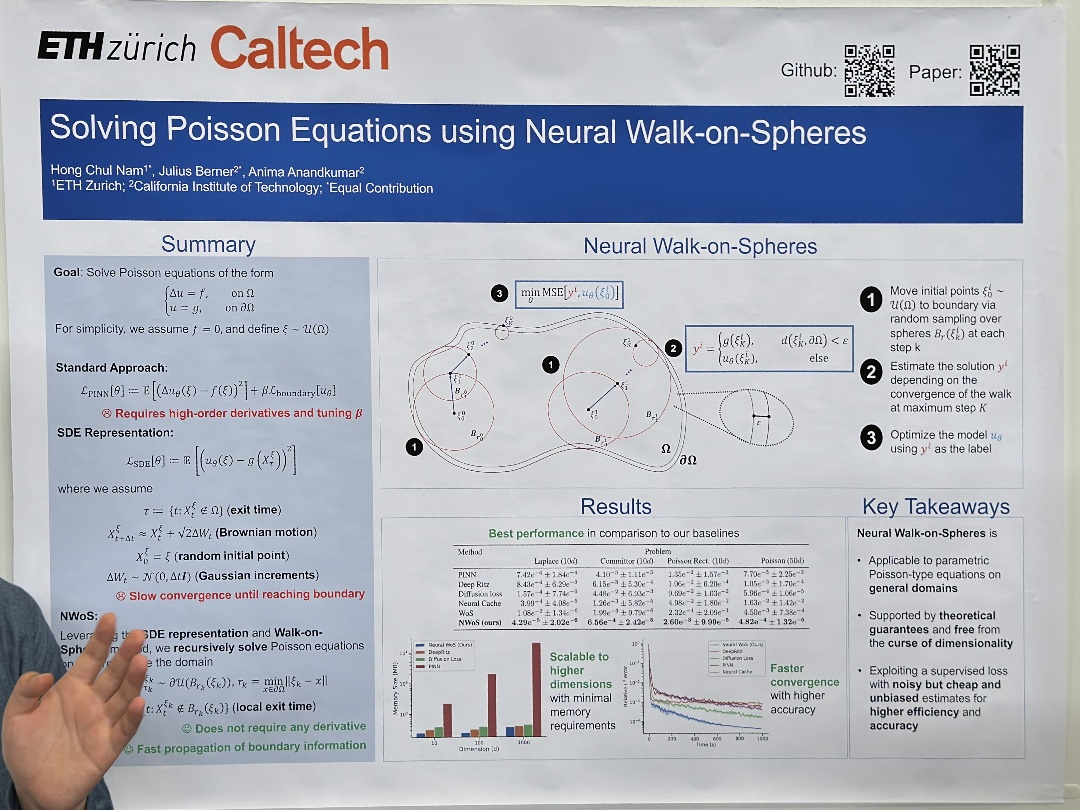
\includegraphics[width=68mm]{out_reduced/IMG_1510.jpeg}} & \textbf{Integral Equation Approach to Stationary Stochastic Counting Process with Independent Increments} 
 \textit{Enzhi Li} 

Solving Poisson Equations using Neural Walk{-}on{-}Spheres

\url{http://arxiv.org/abs/1811.07262v1}\\\raisebox{-\height}{\s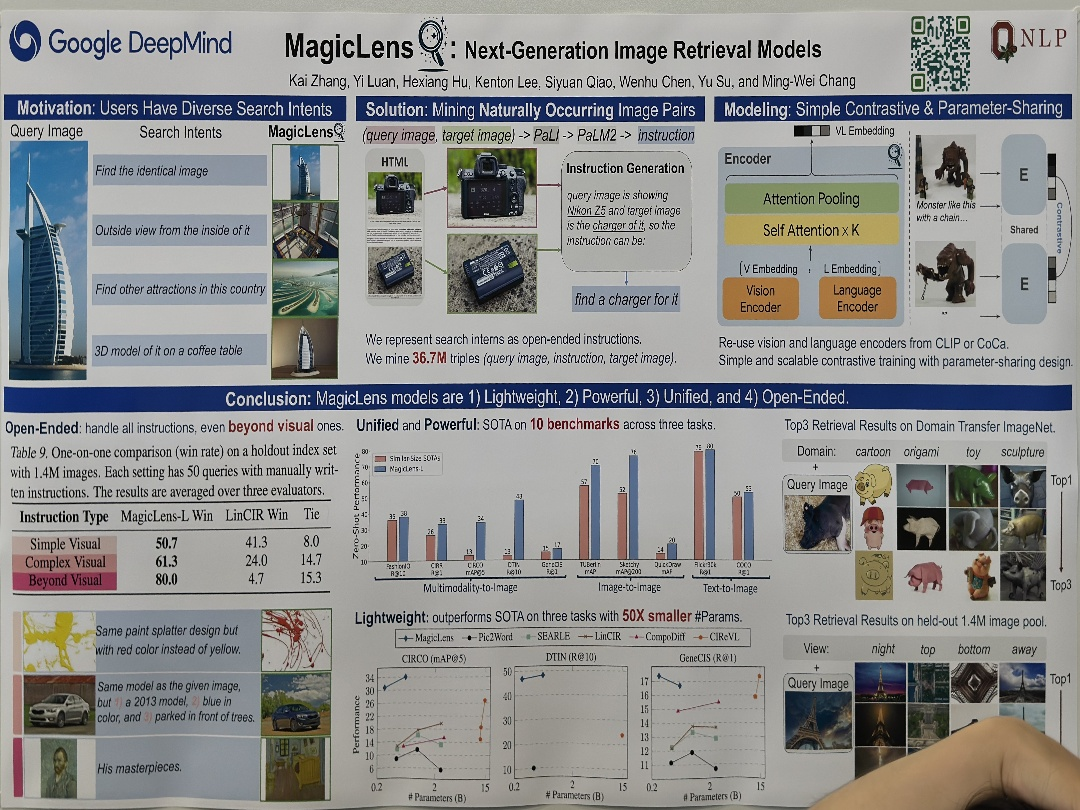
\includegraphics[width=68mm]{out_reduced/IMG_1547.jpeg}} & \textbf{MagicLens: Self{-}Supervised Image Retrieval with Open{-}Ended Instructions} 
 \textit{Kai Zhang,Yi Luan,Hexiang Hu,Kenton Lee,Siyuan Qiao,Wenhu Chen,Yu Su,Ming{-}Wei Chang} 

MagicLens: Next{-}Generation Image Retrieval Models

\url{http://arxiv.org/abs/2403.19651v2}\\\raisebox{-\height}{\s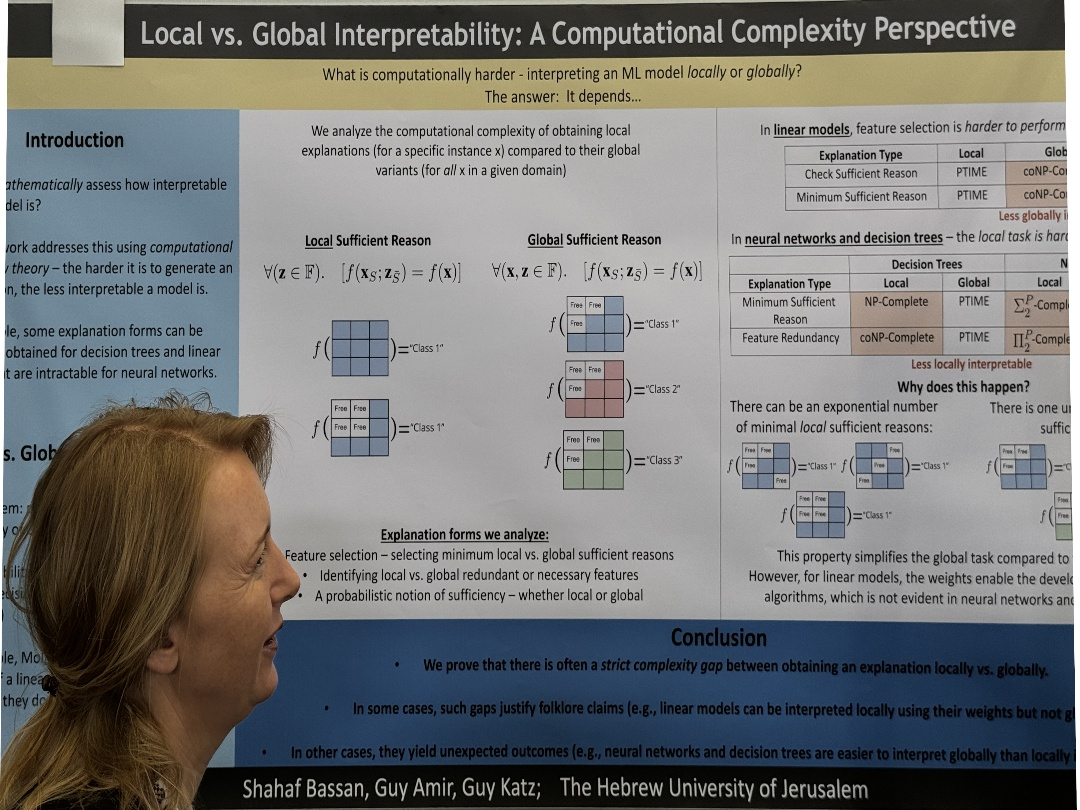
\includegraphics[width=68mm]{out_reduced/IMG_1551.jpeg}} & \textbf{Local vs. Global Interpretability: A Computational Complexity Perspective} 
 \textit{Shahaf Bassan,Guy Amir,Guy Katz} 

Local vs. Global Interpretability: A Computational Complexity Perspective

\url{http://arxiv.org/abs/2406.02981v2}\\\raisebox{-\height}{\s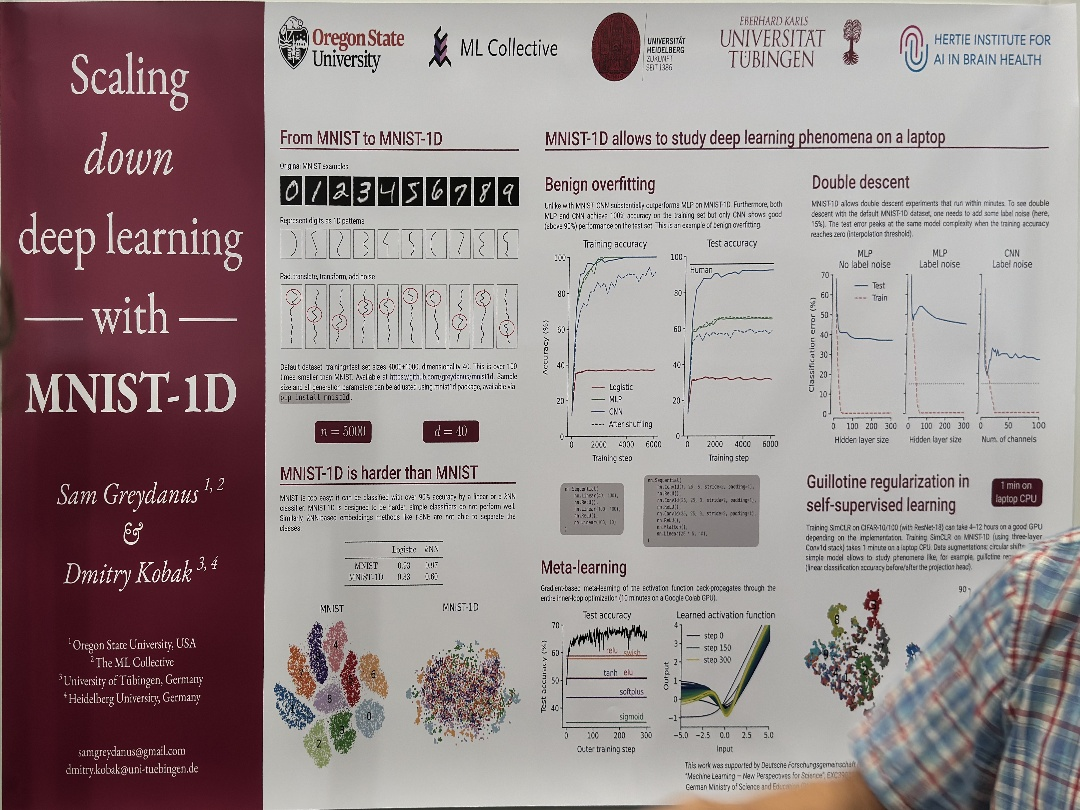
\includegraphics[width=68mm]{out_reduced/IMG_1506.jpeg}} & \textbf{deep learning} 
 \textit{nn. Convid(25, 25, 3, stride=2, padding=1),} 

deep learning

\url{}\\\raisebox{-\height}{\s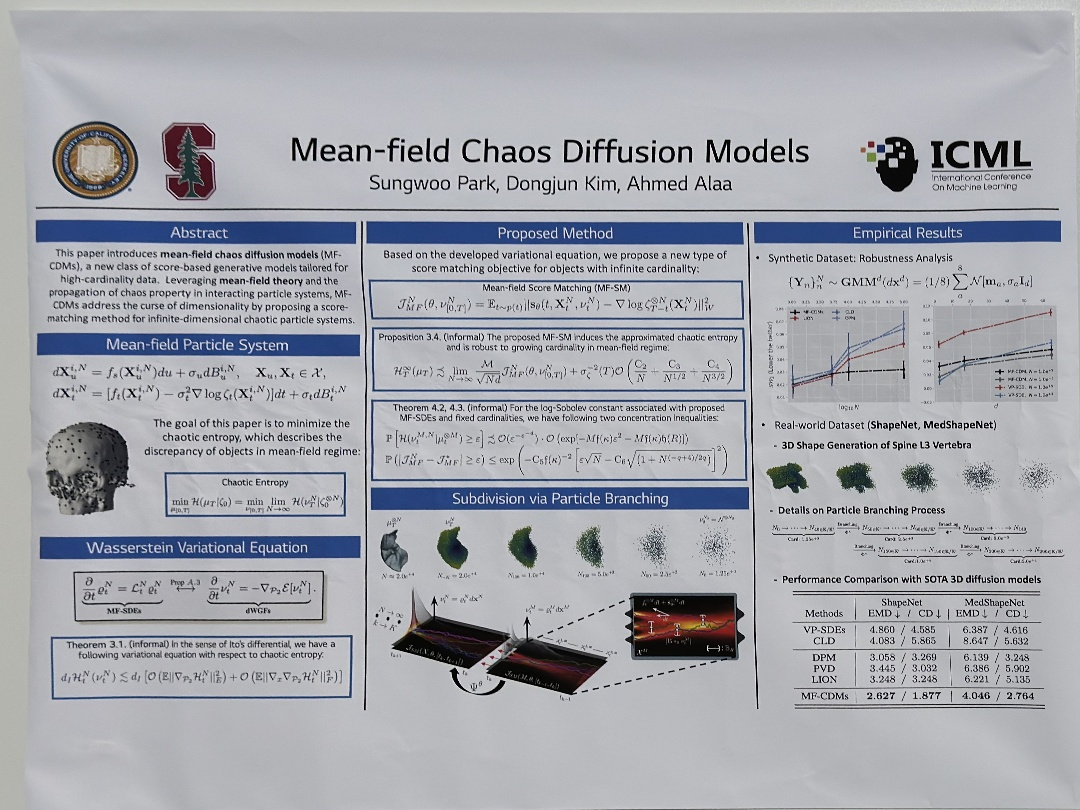
\includegraphics[width=68mm]{out_reduced/IMG_1529.jpeg}} & \textbf{Active matter beyond mean{-}field: Ring{-}kinetic theory for self{-}propelled particles} 
 \textit{Yen{-}Liang Chou,Thomas Ihle} 

Mean{-}field Chaos Diffusion Models

\url{http://dx.doi.org/10.1103/PhysRevE.91.022103}\\\raisebox{-\height}{\s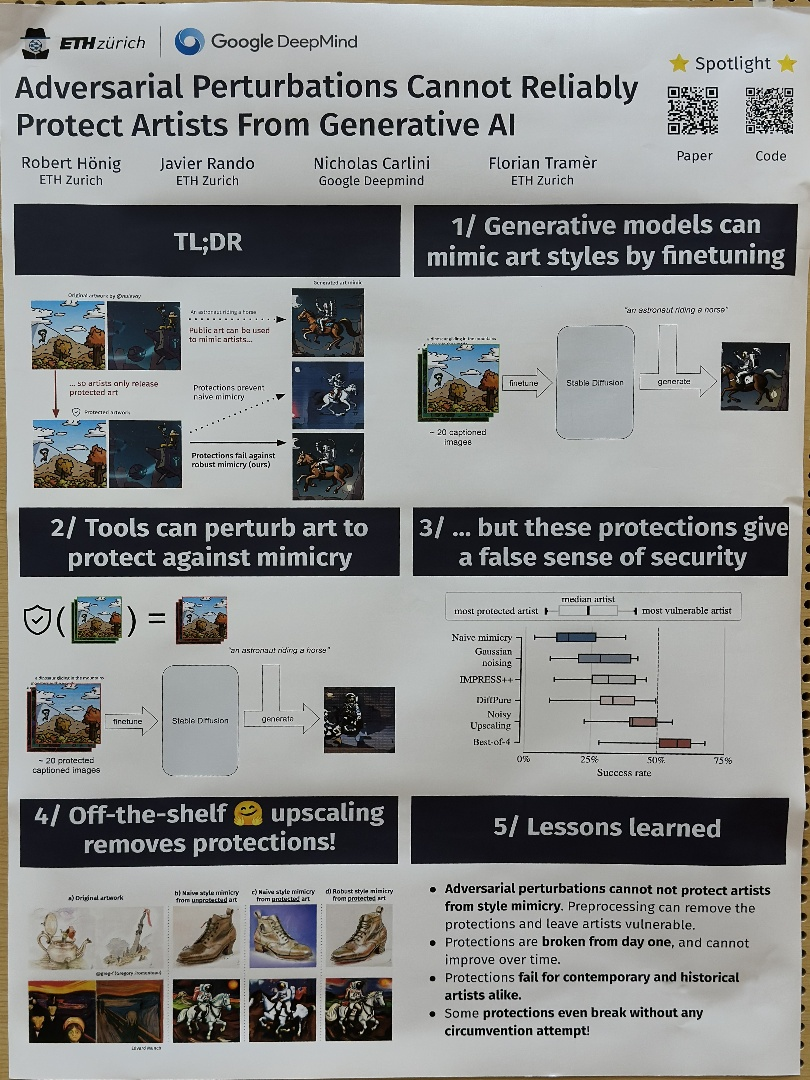
\includegraphics[width=68mm]{out_reduced/IMG_1600.jpeg}} & \textbf{Adversarial Perturbations Cannot Reliably Protect Artists From Generative AI} 
 \textit{Robert Hönig,Javier Rando,Nicholas Carlini,Florian Tramèr} 

Adversarial Perturbations Cannot Reliably

\url{http://arxiv.org/abs/2406.12027v1}\\\raisebox{-\height}{\s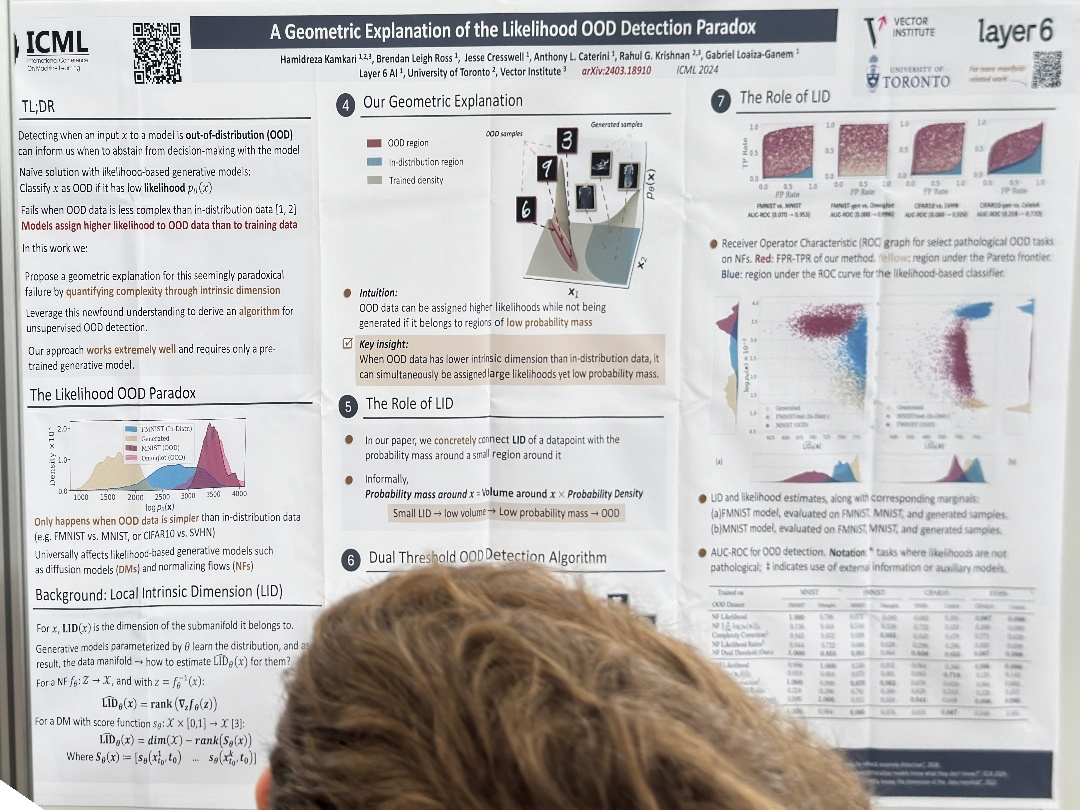
\includegraphics[width=68mm]{out_reduced/IMG_1568.jpeg}} & \textbf{A Geometric Explanation of the Likelihood OOD Detection Paradox} 
 \textit{Hamidreza Kamkari,Brendan Leigh Ross,Jesse C. Cresswell,Anthony L. Caterini,Rahul G. Krishnan,Gabriel Loaiza{-}Ganem} 

A Geometric Explanation of the Likelihood OOD Detection Paradox

\url{http://arxiv.org/abs/2403.18910v2}\\\raisebox{-\height}{\s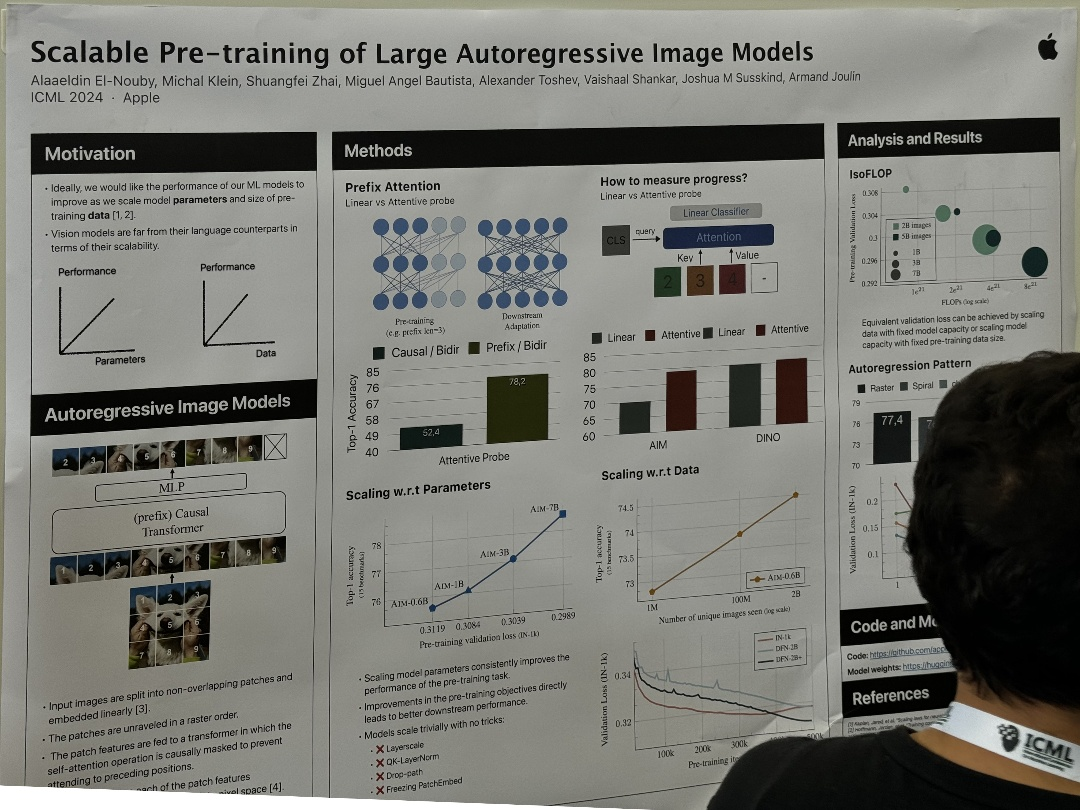
\includegraphics[width=68mm]{out_reduced/IMG_1552.jpeg}} & \textbf{Scalable Pre{-}training of Large Autoregressive Image Models} 
 \textit{Alaaeldin El{-}Nouby,Michal Klein,Shuangfei Zhai,Miguel Angel Bautista,Alexander Toshev,Vaishaal Shankar,Joshua M Susskind,Armand Joulin} 

Scalable Pre{-}training of Large Autoregressive Image Models

\url{http://arxiv.org/abs/2401.08541v1}\\\raisebox{-\height}{\s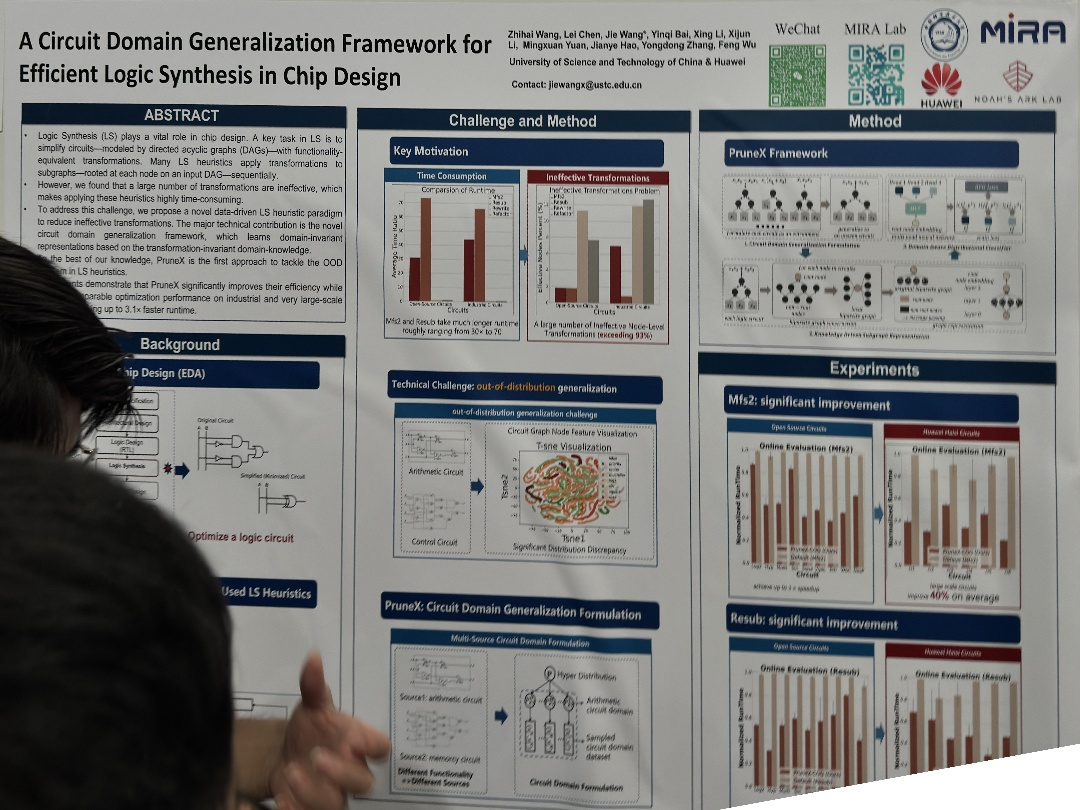
\includegraphics[width=68mm]{out_reduced/IMG_1505.jpeg}} & \textbf{A Circuit Domain Generalization Framework for Efficient Logic Synthesis in Chip Design} 
 \textit{Zhihai Wang,Lei Chen,Jie Wang,Xing Li,Yinqi Bai,Xijun Li,Mingxuan Yuan,Jianye Hao,Yongdong Zhang,Feng Wu} 

Efficient Logic Synthesis in Chip Design

\url{http://arxiv.org/abs/2309.03208v1}\\\raisebox{-\height}{\s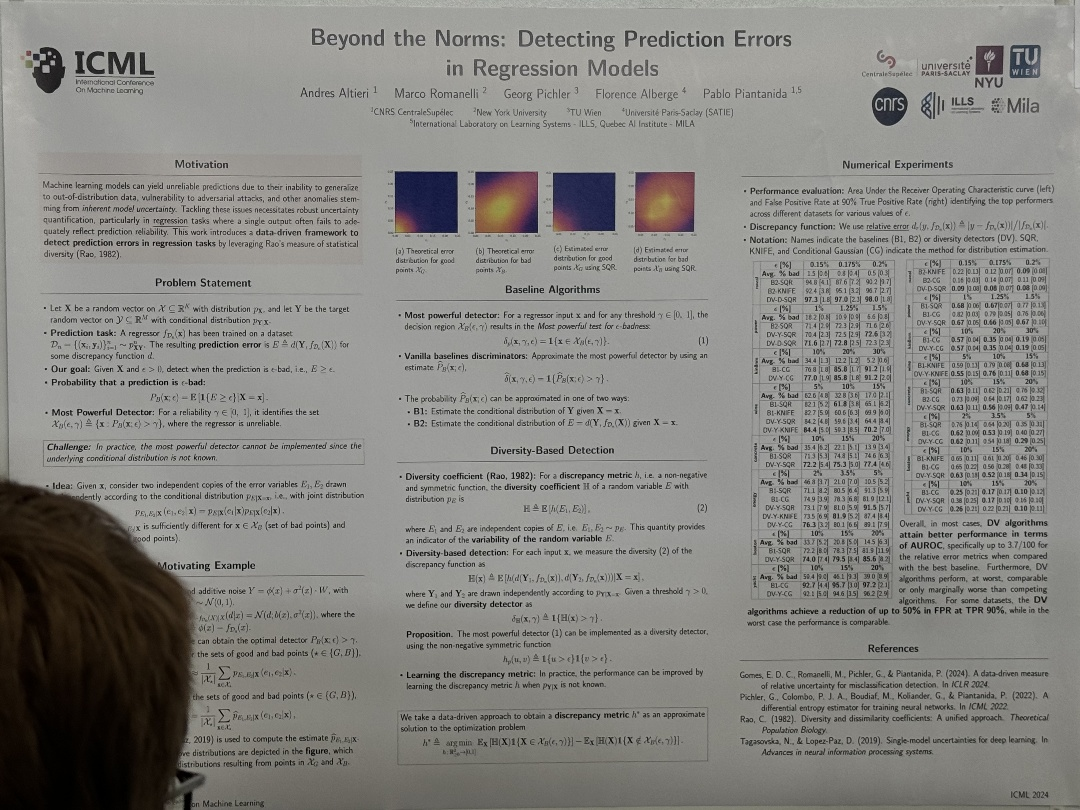
\includegraphics[width=68mm]{out_reduced/IMG_1533.jpeg}} & \textbf{Foliations on double{-}twisted products} 
 \textit{André Gomes} 

2122202171071721

\url{http://arxiv.org/abs/1101.5730v1}\\\raisebox{-\height}{\s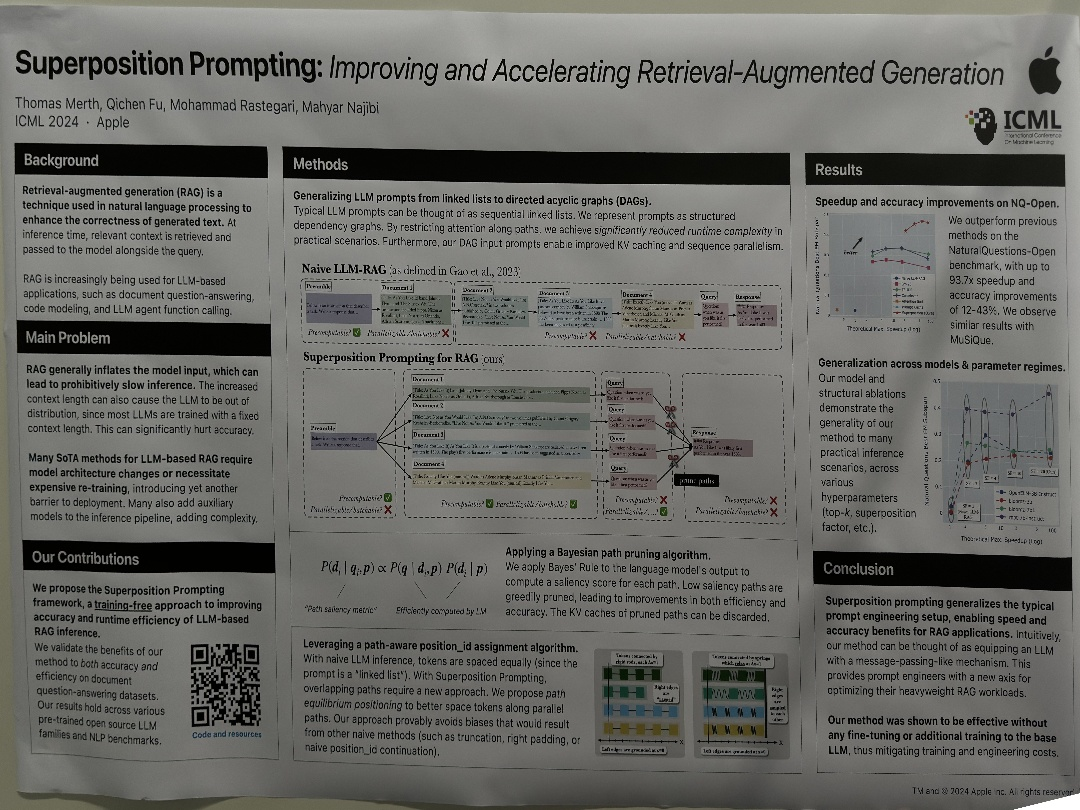
\includegraphics[width=68mm]{out_reduced/IMG_1564.jpeg}} & \textbf{Superpositions of thermalisation states in relativistic quantum field theory} 
 \textit{Joshua Foo,Magdalena Zych} 

Superposition Prompting: Improving and Accelerating Retrieval{-}Augmented Generation

\url{http://arxiv.org/abs/2307.02593v1}\\\raisebox{-\height}{\s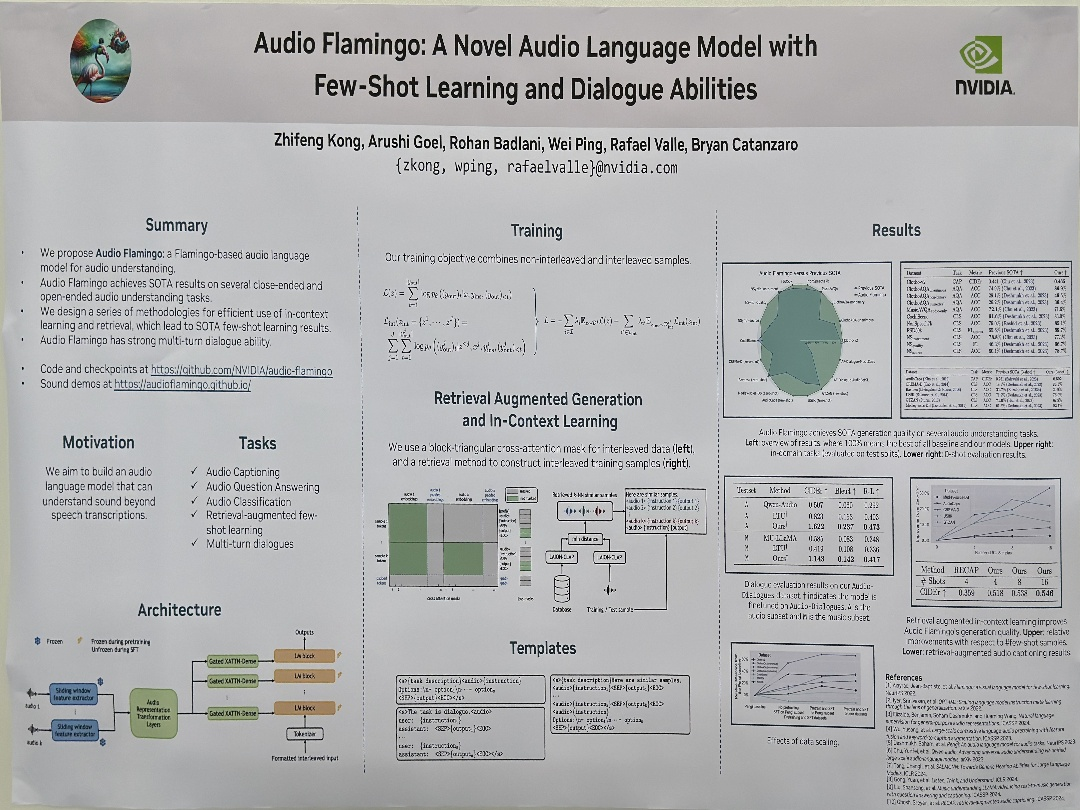
\includegraphics[width=68mm]{out_reduced/IMG_1509.jpeg}} & \textbf{Zero{-}shot audio captioning with audio{-}language model guidance and audio context keywords} 
 \textit{Leonard Salewski,Stefan Fauth,A. Sophia Koepke,Zeynep Akata} 

Audio Flamingo: A Novel Audio Language Model with

\url{http://arxiv.org/abs/2311.08396v1}\\\raisebox{-\height}{\s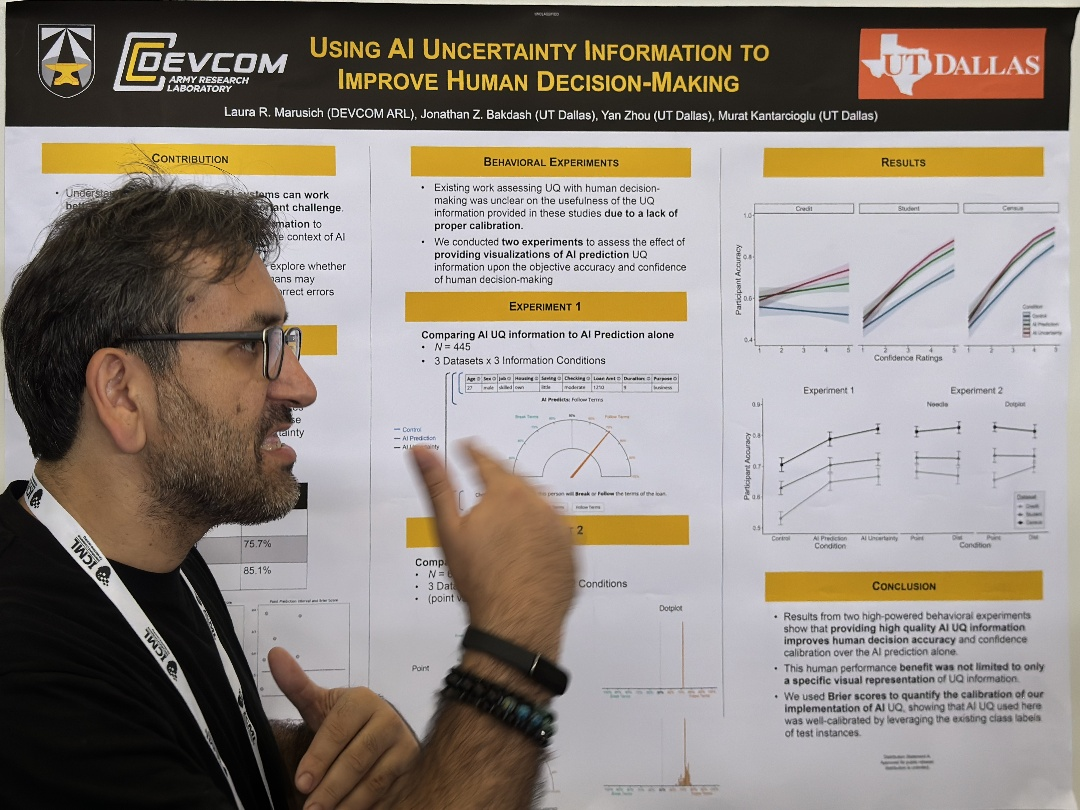
\includegraphics[width=68mm]{out_reduced/IMG_1508.jpeg}} & \textbf{Using AI Uncertainty Quantification to Improve Human Decision{-}Making} 
 \textit{Laura R. Marusich,Jonathan Z. Bakdash,Yan Zhou,Murat Kantarcioglu} 

Laura R. Marusich (DEVCOM ARL), Jonathan Z. Bakdash (UT Dallas), Yan Zhou (UT Dallas), Murat Kantarcioglu (UT Dallas)

\url{http://arxiv.org/abs/2309.10852v2}\\\raisebox{-\height}{\s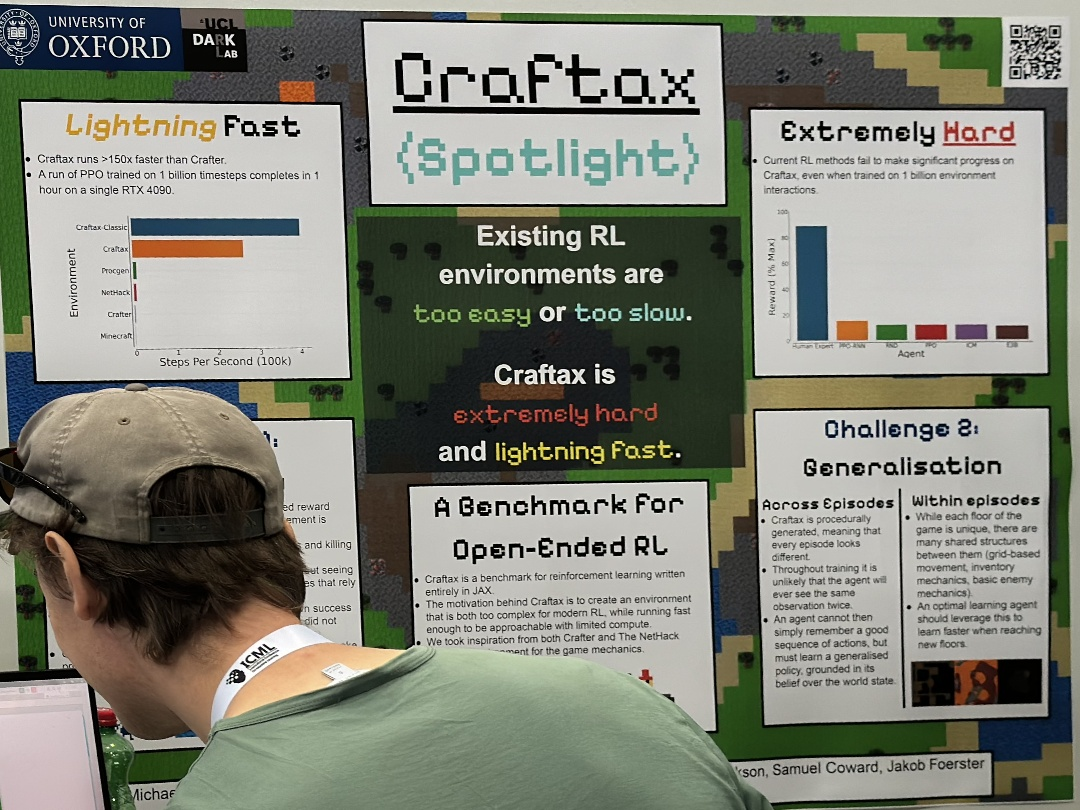
\includegraphics[width=68mm]{out_reduced/IMG_1549.jpeg}} & \textbf{About Geometry and Initial Phase of Cloud{-}to{-}Ground Lightning} 
 \textit{Aleš Berkopec} 

Crafto

\url{http://arxiv.org/abs/1602.02496v1}\\\raisebox{-\height}{\s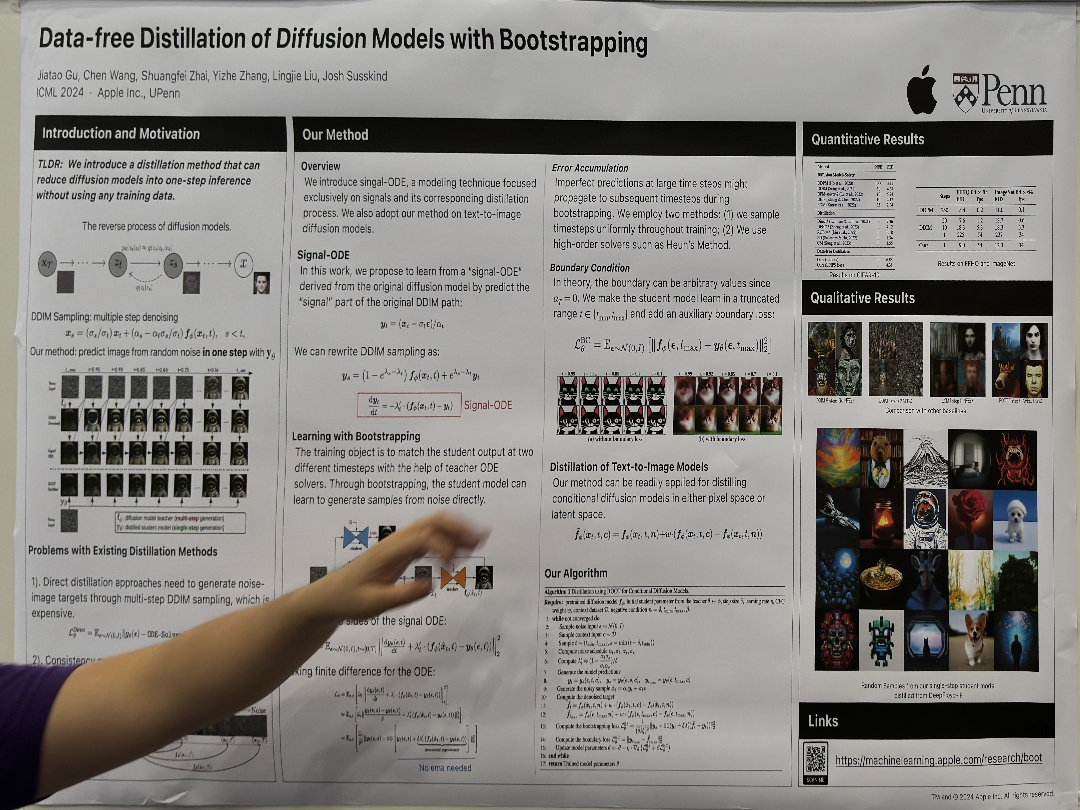
\includegraphics[width=68mm]{out_reduced/IMG_1553.jpeg}} & \textbf{Data{-}free Distillation of Diffusion Models with Bootstrapping} 
 \textit{fo (xt, t, c) = fox, t, n) +w. (fo (xt, t, c) {-} foxt, t, n))} 

Data{-}free Distillation of Diffusion Models with Bootstrapping

\url{}\\\raisebox{-\height}{\s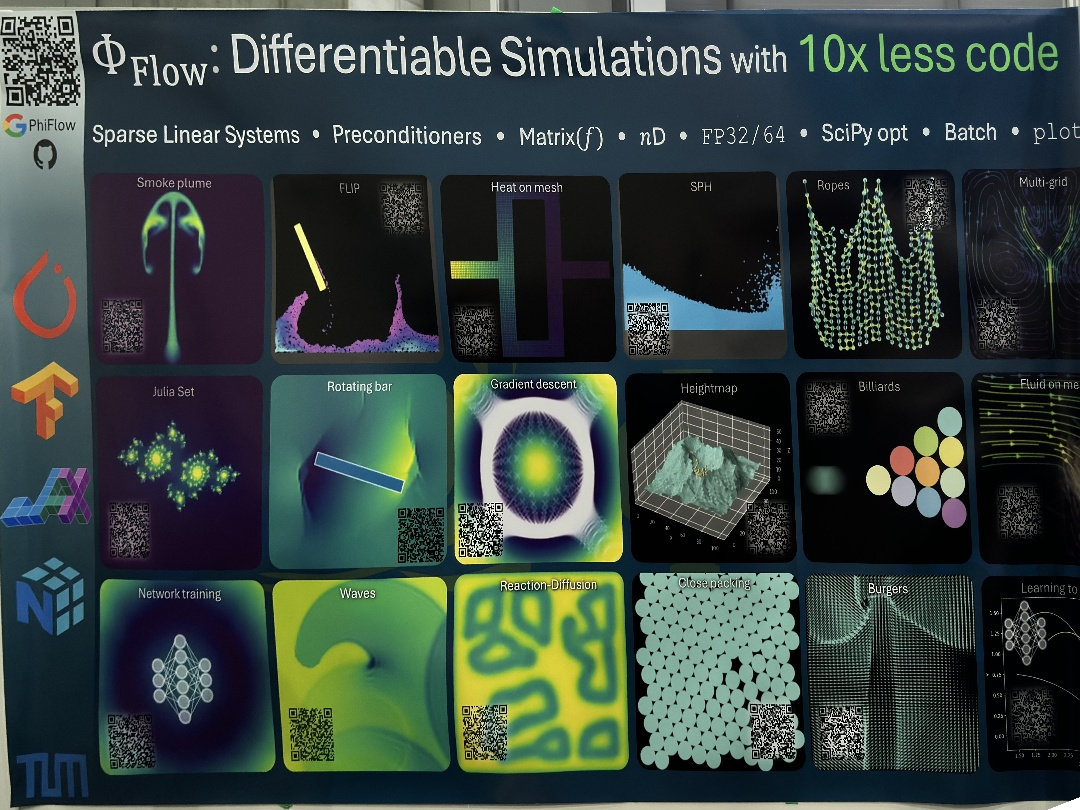
\includegraphics[width=68mm]{out_reduced/IMG_1545.jpeg}} & \textbf{Measuring the Earth's Synchrotron Emission from Radiation Belts with a Lunar Near Side Radio Array} 
 \textit{Alexander Hegedus,Quentin Nenon,Antoine Brunet,Justin Kasper,Angelica Sicard,Baptiste Cecconi,Robert MacDowall,Daniel Baker} 

\$ Flow: Differentiable Simulations with 10x less code

\url{http://dx.doi.org/10.1029/2019RS006891}\\\raisebox{-\height}{\s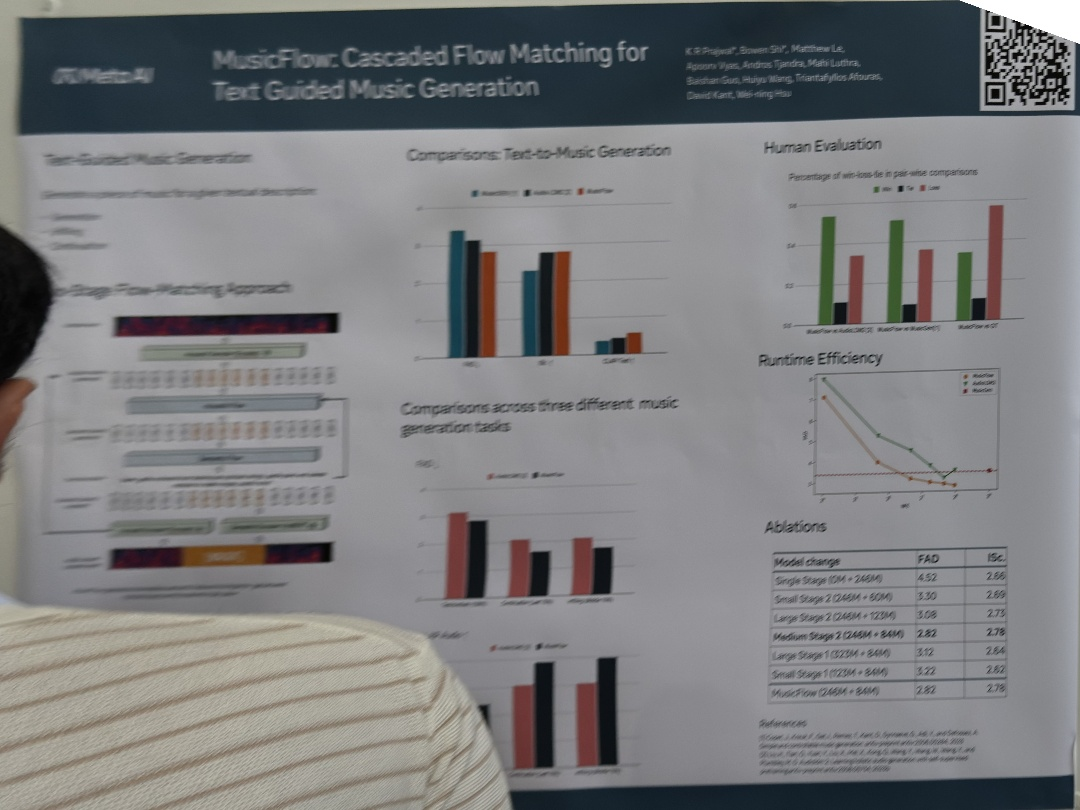
\includegraphics[width=68mm]{out_reduced/IMG_1512.jpeg}} & \textbf{A double{-}layer Boussinesq{-}type model for highly nonlinear and dispersive waves} 
 \textit{Florent Chazel,Michel Benoit,Alexandre Ern,Serge Piperno} 

MusicFlow: Cascaded Flow Matching for

\url{http://dx.doi.org/10.1098/rspa.2008.0508}\\\raisebox{-\height}{\s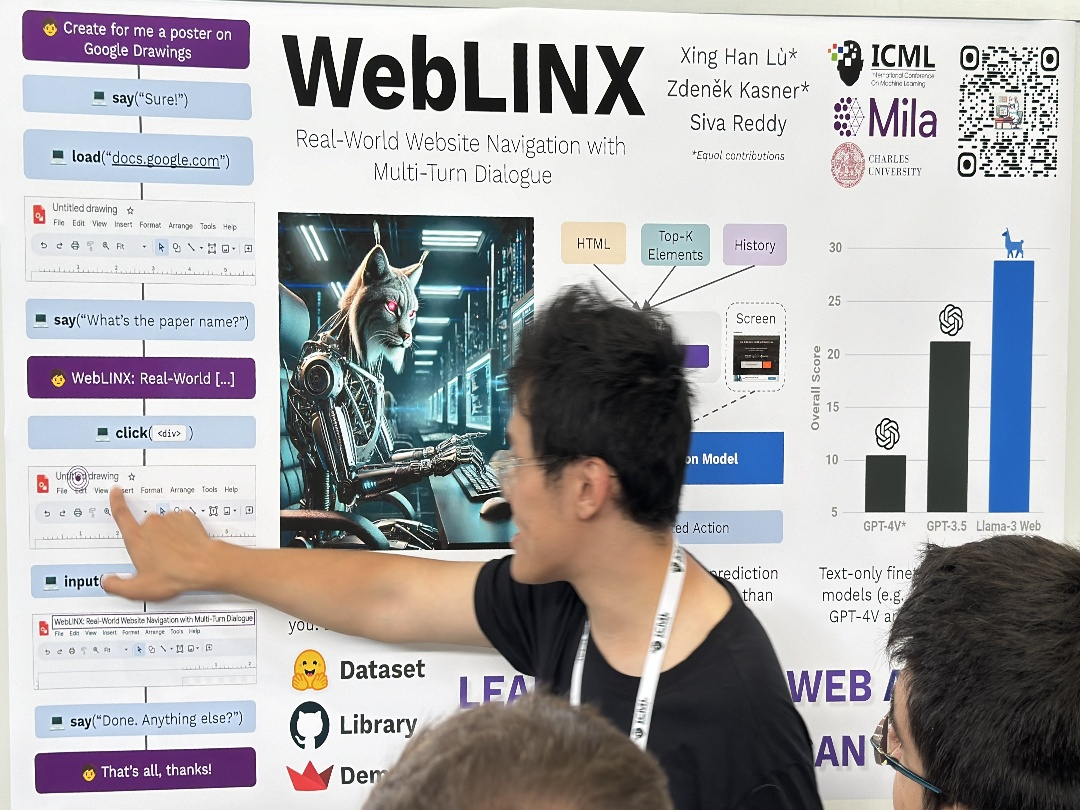
\includegraphics[width=68mm]{out_reduced/IMG_1569.jpeg}} & \textbf{WebLINX} 
 \textit{WebLINX: Real{-}World {[}...{]}} 

WebLINX

\url{}\\\raisebox{-\height}{\s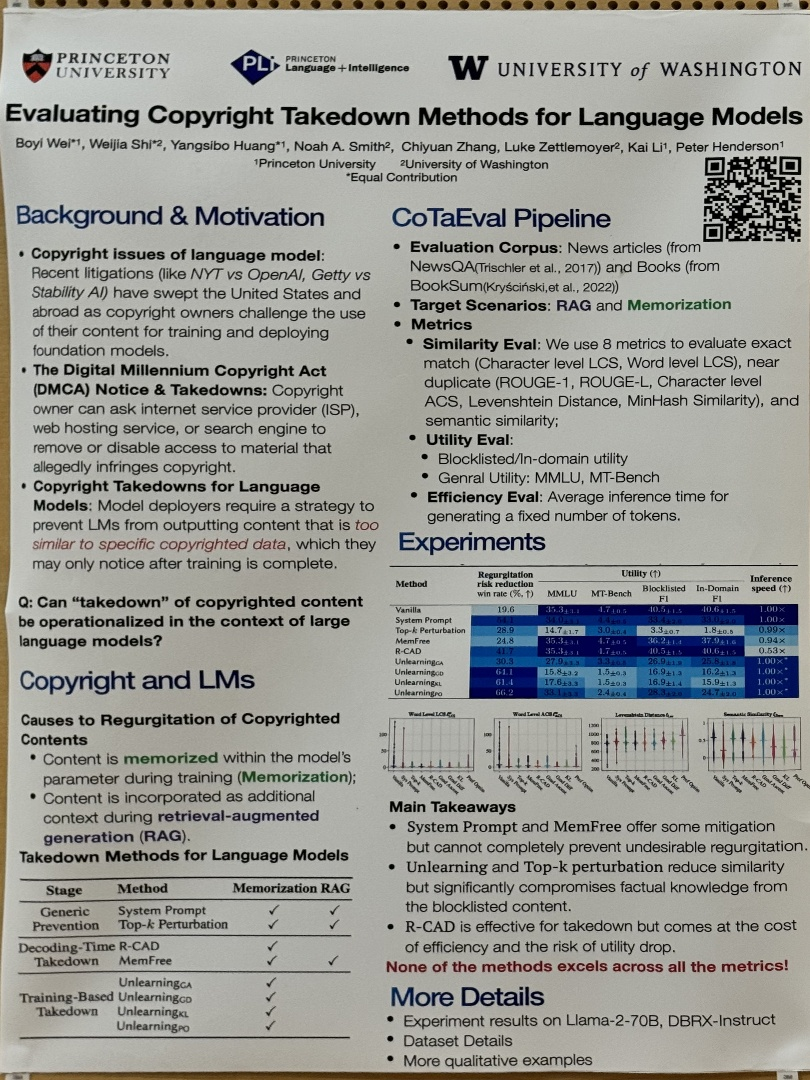
\includegraphics[width=68mm]{out_reduced/IMG_1601.jpeg}} & \textbf{Evaluating Copyright Takedown Methods for Language Models} 
 \textit{Boyi Wei,Weijia Shi,Yangsibo Huang,Noah A. Smith,Chiyuan Zhang,Luke Zettlemoyer,Kai Li,Peter Henderson} 

Evaluating Copyright Takedown Methods for Language Models

\url{http://arxiv.org/abs/2406.18664v3}\\\raisebox{-\height}{\s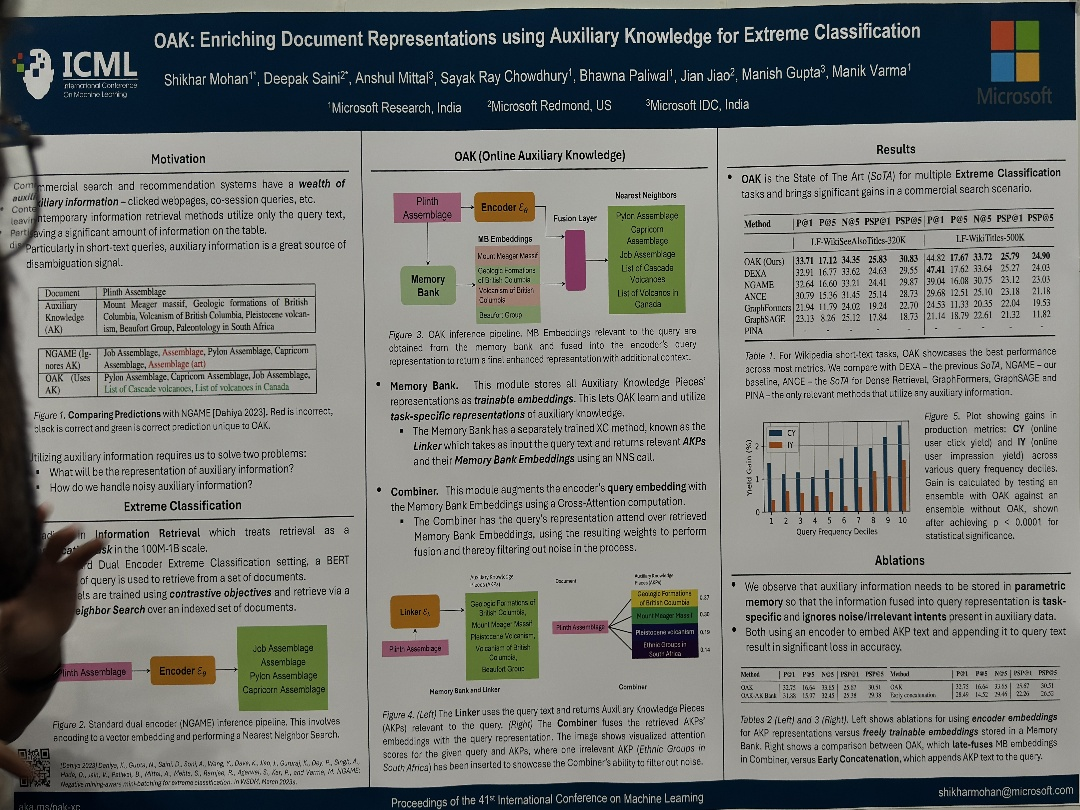
\includegraphics[width=68mm]{out_reduced/IMG_1535.jpeg}} & \textbf{Auxiliary Knowledge{-}Induced Learning for Automatic Multi{-}Label Medical Document Classification} 
 \textit{Xindi Wang,Robert E. Mercer,Frank Rudzicz} 

OAK: Enriching Document Representations using Auxiliary Knowledge for Extreme Classification

\url{http://arxiv.org/abs/2405.19084v1}\\\raisebox{-\height}{\s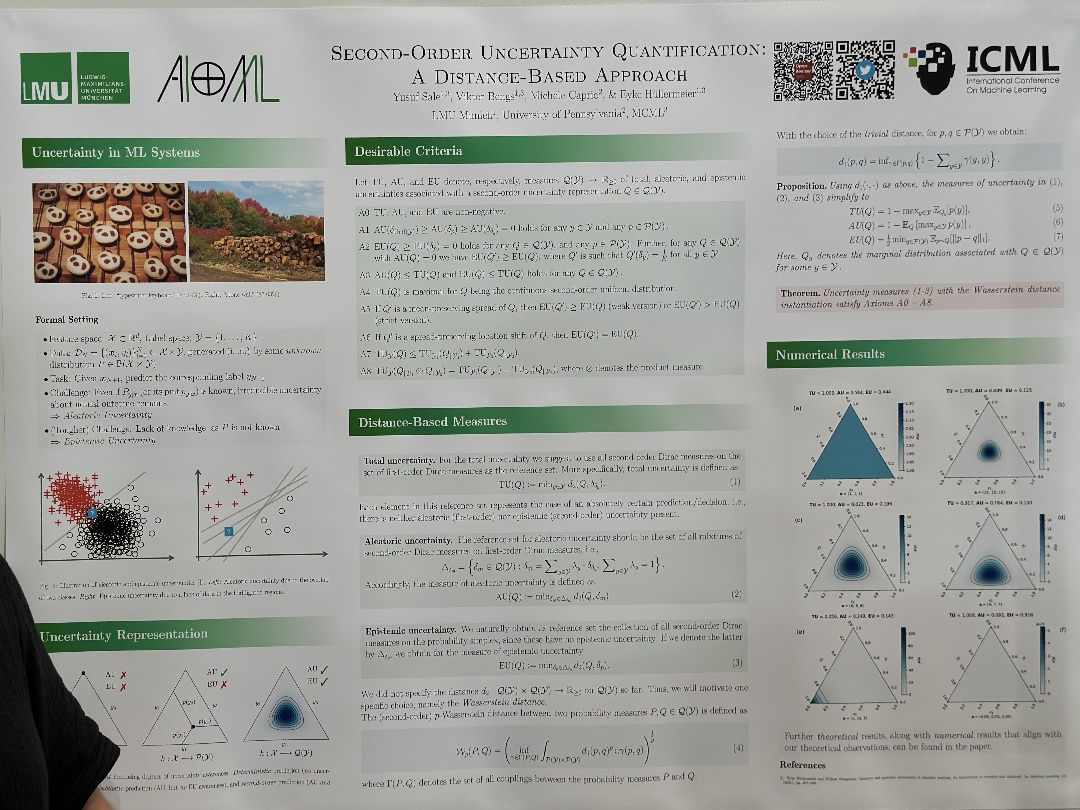
\includegraphics[width=68mm]{out_reduced/IMG_1562.jpeg}} & \textbf{Power{-}Law distributions and Fisher's information measure} 
 \textit{F. Pennini,A. Plastino} 

SECOND{-}ORDER UNCERTAINTY QUANTIFICATION:

\url{http://dx.doi.org/10.1016/j.physa.2003.10.076}\\\raisebox{-\height}{\s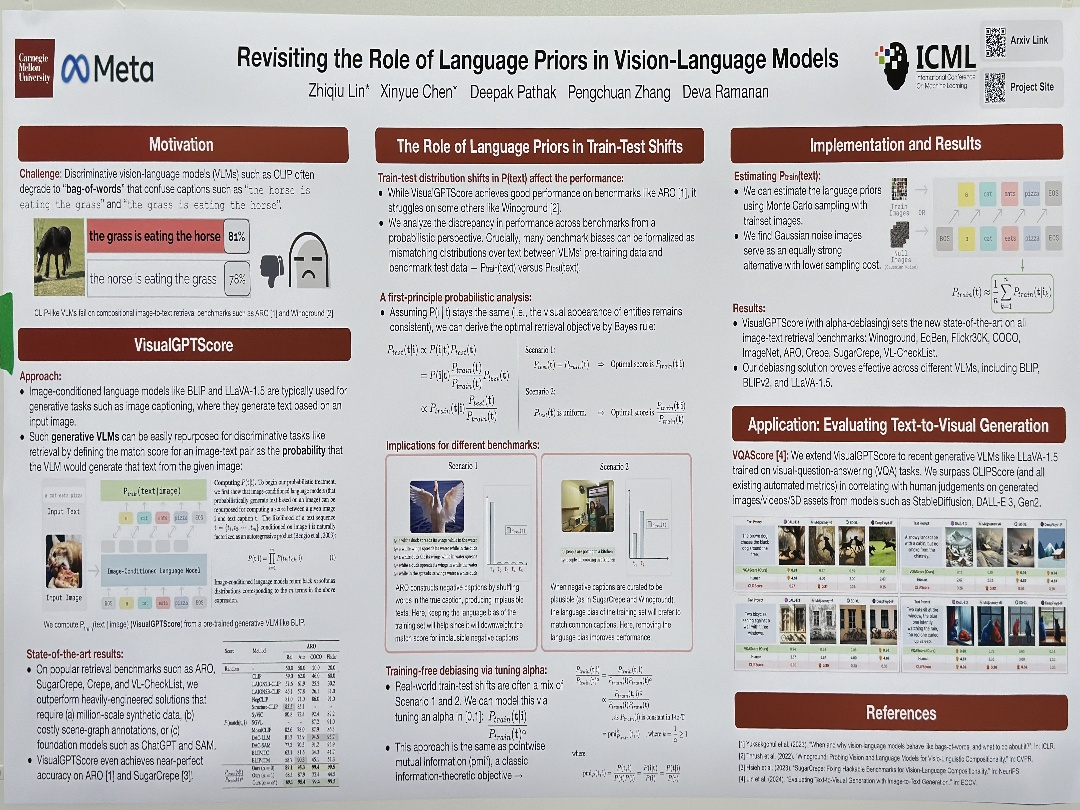
\includegraphics[width=68mm]{out_reduced/IMG_1558.jpeg}} & \textbf{Revisiting the Role of Language Priors in Vision{-}Language Models} 
 \textit{{[}1{]} Yuksekgonul et al. (2023). "When and why vision{-}language models behave like bags{-}of{-}words, and what to do about it?", In: ICLR.} 

Revisiting the Role of Language Priors in Vision{-}Language Models

\url{}\\\raisebox{-\height}{\s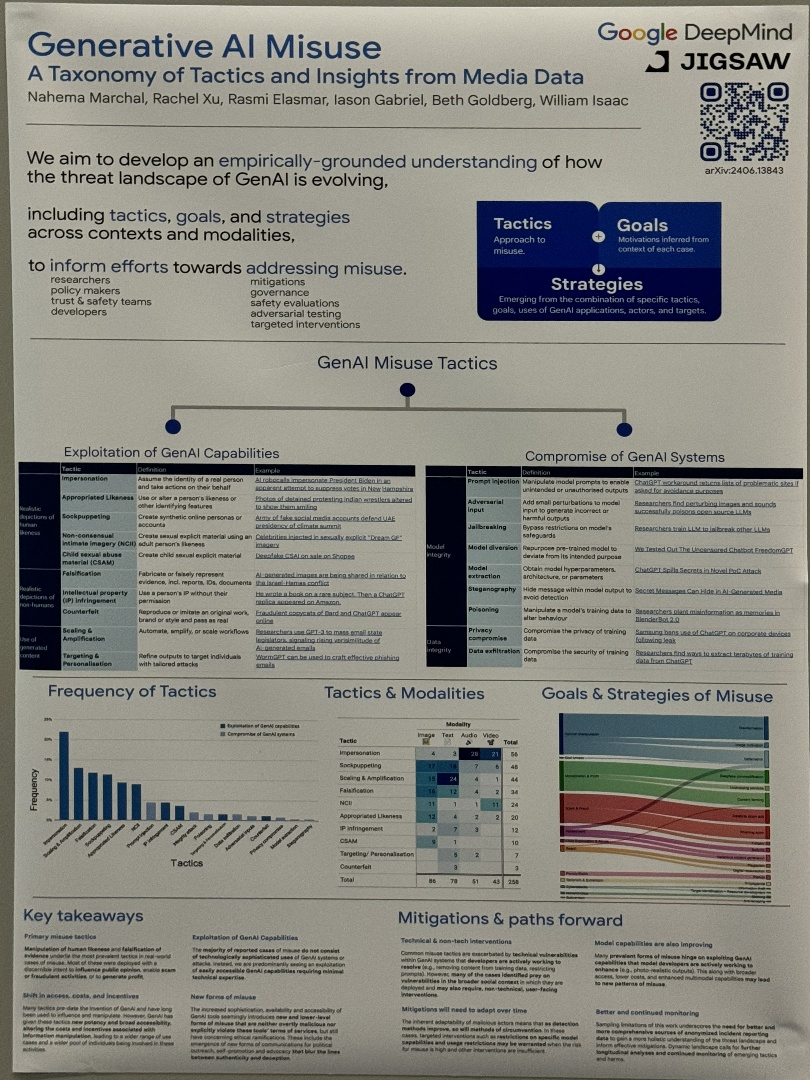
\includegraphics[width=68mm]{out_reduced/IMG_1597.jpeg}} & \textbf{Generative AI Misuse: A Taxonomy of Tactics and Insights from Real{-}World Data} 
 \textit{Nahema Marchal,Rachel Xu,Rasmi Elasmar,Iason Gabriel,Beth Goldberg,William Isaac} 

A Taxonomy of Tactics and Insights from Media Data

\url{http://arxiv.org/abs/2406.13843v2}\\\raisebox{-\height}{\s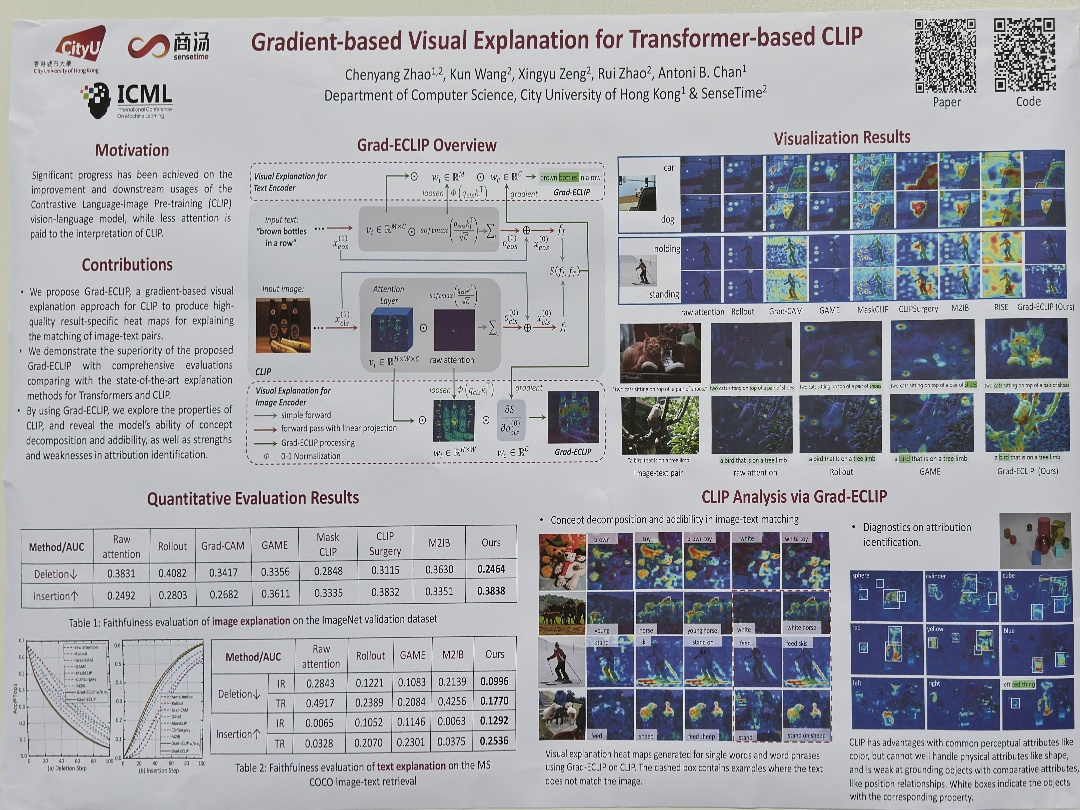
\includegraphics[width=68mm]{out_reduced/IMG_1539.jpeg}} & \textbf{RCA: Region Conditioned Adaptation for Visual Abductive Reasoning} 
 \textit{Hao Zhang,Yeo Keat Ee,Basura Fernando} 

Gradient{-}based Visual Explanation for Transformer{-}based CLIP

\url{http://arxiv.org/abs/2303.10428v4}\\\raisebox{-\height}{\s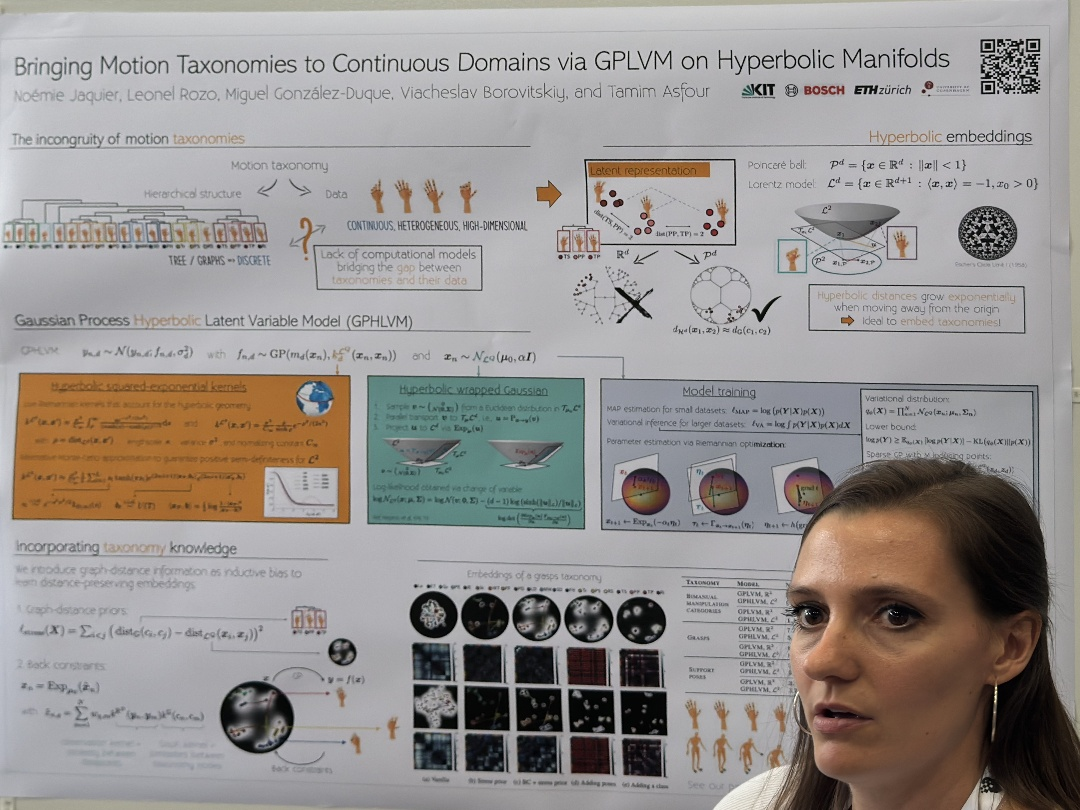
\includegraphics[width=68mm]{out_reduced/IMG_1515.jpeg}} & \textbf{Bringing motion taxonomies to continuous domains via GPLVM on hyperbolic manifolds} 
 \textit{Noémie Jaquier,Leonel Rozo,Miguel González{-}Duque,Viacheslav Borovitskiy,Tamim Asfour} 

Bringing Motion Taxonomies to Continuous Domains via GPLVM on Hyperbolic Manifolds

\url{http://arxiv.org/abs/2210.01672v4}\\\raisebox{-\height}{\s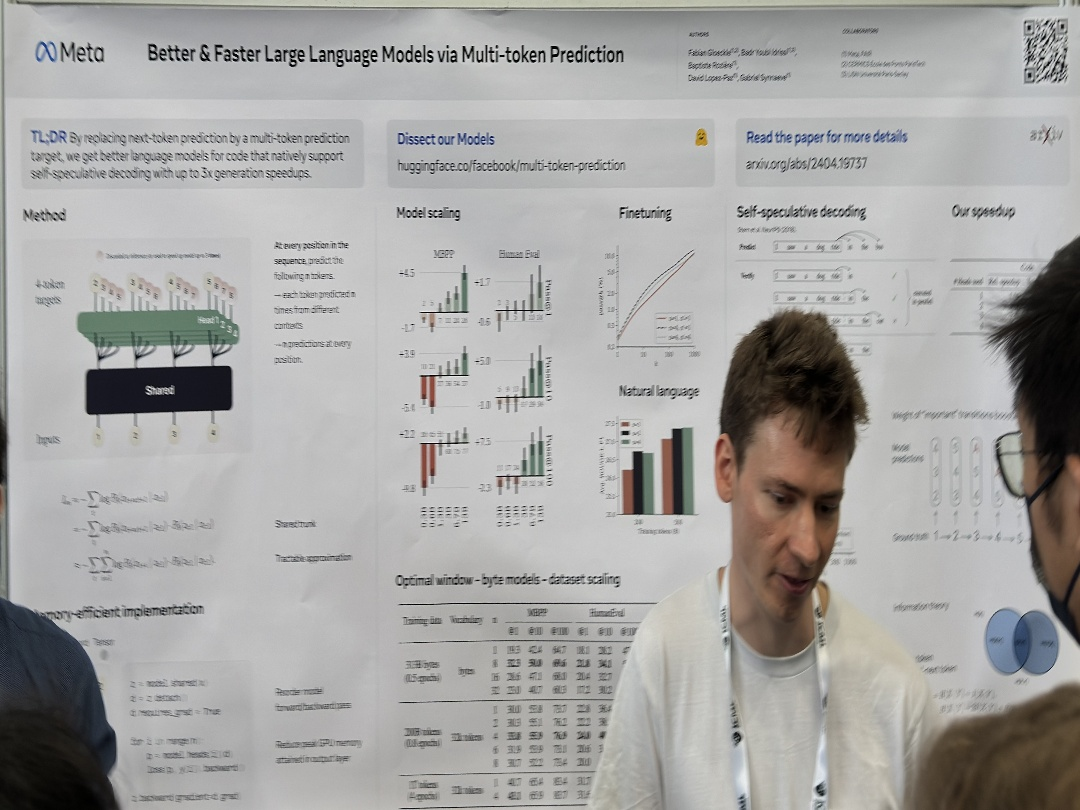
\includegraphics[width=68mm]{out_reduced/IMG_1542.jpeg}} & \textbf{Better \& Faster Large Language Models via Multi{-}token Prediction} 
 \textit{Fabian Gloeckle,Badr Youbi Idrissi,Baptiste Rozière,David Lopez{-}Paz,Gabriel Synnaeve} 

Better \& Faster Large Language Models via Multi{-}token Prediction

\url{http://arxiv.org/abs/2404.19737v1}\\\raisebox{-\height}{\s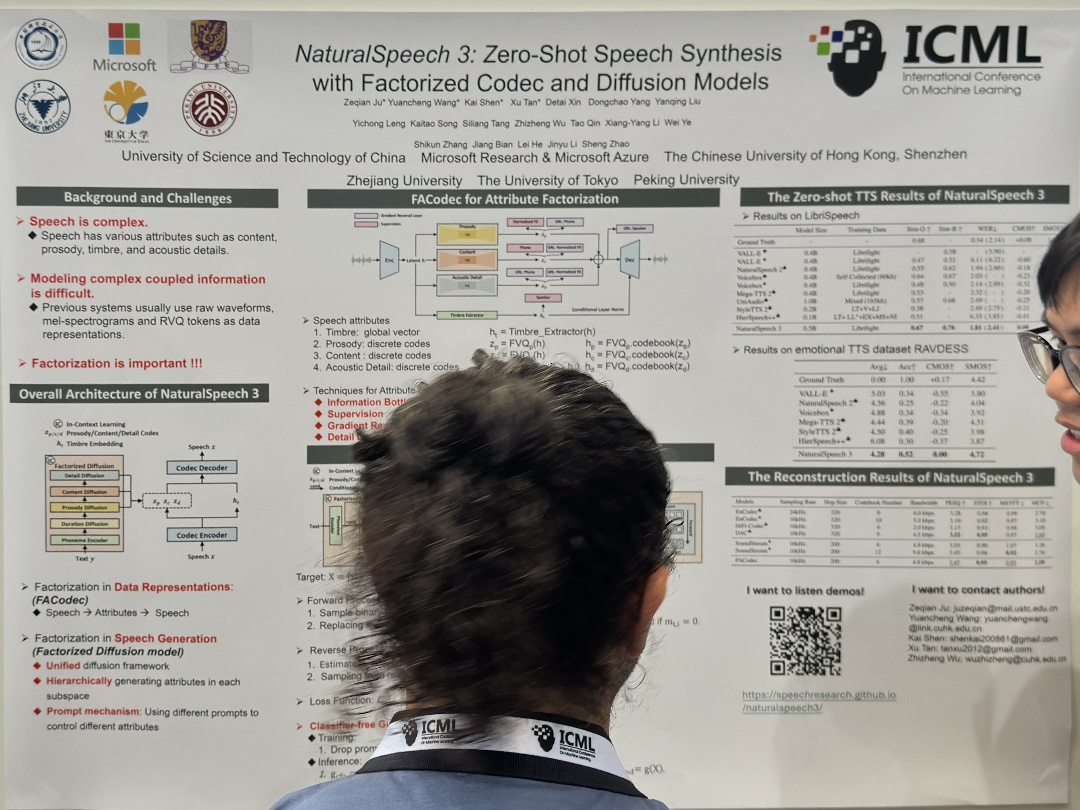
\includegraphics[width=68mm]{out_reduced/IMG_1543.jpeg}} & \textbf{TJ{-}FlyingFish: Design and Implementation of an Aerial{-}Aquatic Quadrotor with Tiltable Propulsion Units} 
 \textit{Xuchen Liu,Minghao Dou,Dongyue Huang,Biao Wang,Jinqiang Cui,Qinyuan Ren,Lihua Dou,Zhi Gao,Jie Chen,Ben M. Chen} 

University of Science and Technology of China Microsoft Research \& Microsoft Azure The Chinese University of Hong Kong, Shenzhen

\url{http://arxiv.org/abs/2301.12344v2}\\\raisebox{-\height}{\s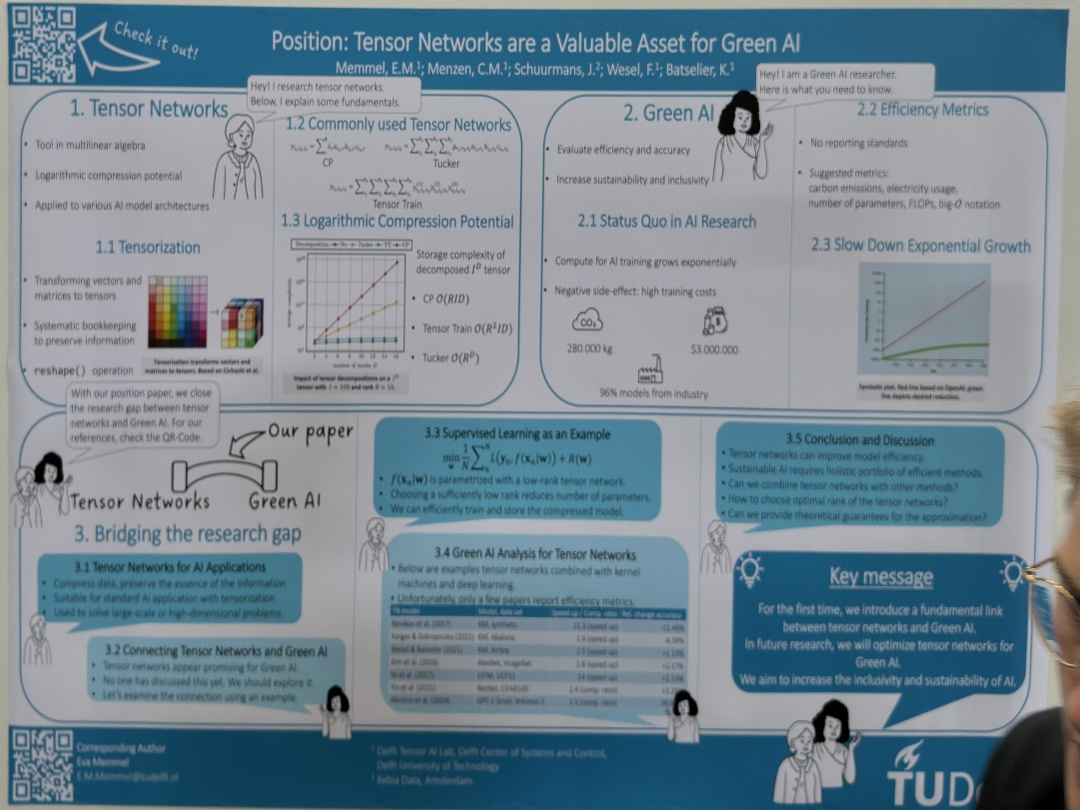
\includegraphics[width=68mm]{out_reduced/IMG_1514.jpeg}} & \textbf{Position: Tensor Networks are a Valuable Asset for Green AI} 
 \textit{Eva Memmel,Clara Menzen,Jetze Schuurmans,Frederiek Wesel,Kim Batselier} 

Position: Tensor Networks are a Valuable Asset for Green Al

\url{http://arxiv.org/abs/2205.12961v2}\\\raisebox{-\height}{\s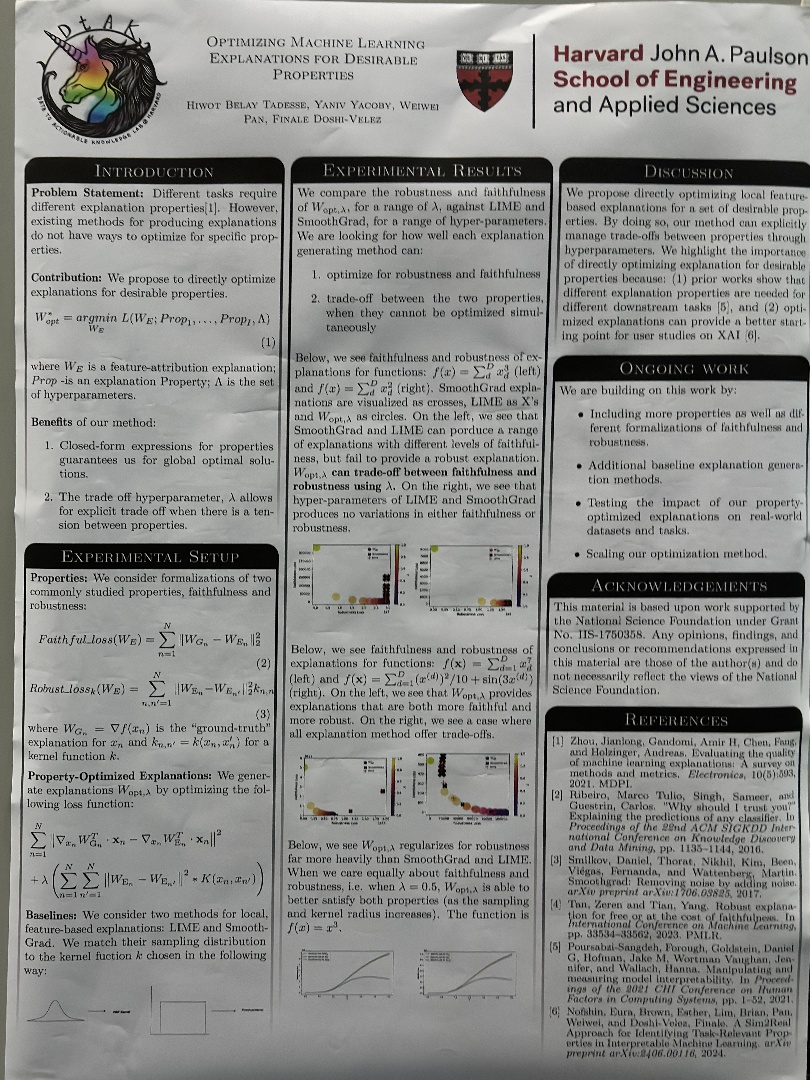
\includegraphics[width=68mm]{out_reduced/IMG_1596.jpeg}} & \textbf{School of Engineering} 
 \textit{{[}1) Zhou, Jianlong, Gandomi, Amir H, Chen, Fang,} 

School of Engineering

\url{}\\\raisebox{-\height}{\s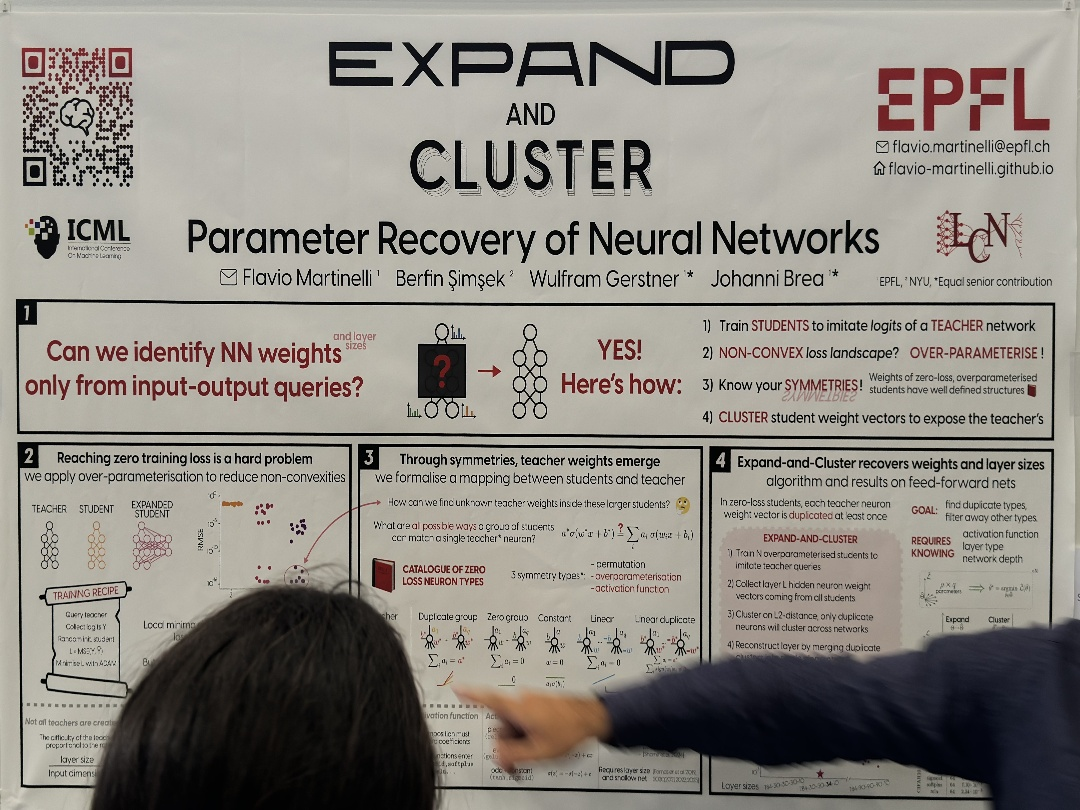
\includegraphics[width=68mm]{out_reduced/IMG_1559.jpeg}} & \textbf{Dual Convexified Convolutional Neural Networks} 
 \textit{Site Bai,Chuyang Ke,Jean Honorio} 

Parameter Recovery of Neural Networks

\url{http://arxiv.org/abs/2205.14056v2}\\\raisebox{-\height}{\s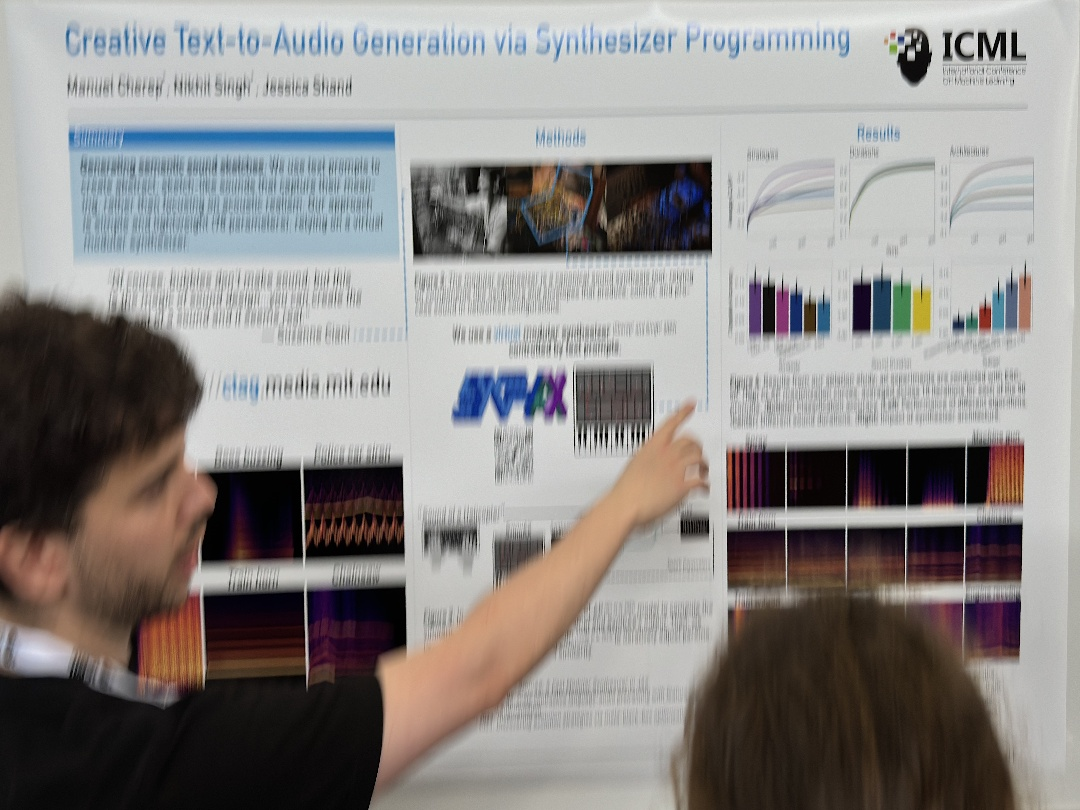
\includegraphics[width=68mm]{out_reduced/IMG_1518.jpeg}} & \textbf{Luban: Building Open{-}Ended Creative Agents via Autonomous Embodied Verification} 
 \textit{Yuxuan Guo,Shaohui Peng,Jiaming Guo,Di Huang,Xishan Zhang,Rui Zhang,Yifan Hao,Ling Li,Zikang Tian,Mingju Gao,Yutai Li,Yiming Gan,Shuai Liang,Zihao Zhang,Zidong Du,Qi Guo,Xing Hu,Yunji Chen} 

Creative Text{-}to{-}Audio Generation Via Synthesizer Programming

\url{http://arxiv.org/abs/2405.15414v1}\\\raisebox{-\height}{\s\includegraphics[width=68mm]{out_reduced/IMG_1534.jpeg}} & \textbf{A Survey on Trustworthy Edge Intelligence: From Security and Reliability To Transparency and Sustainability} 
 \textit{Xiaojie Wang,Beibei Wang,Yu Wu,Zhaolong Ning,Song Guo,Fei Richard Yu} 

TRUSTWORTHY ACTIONABLE PERTURBATIONS

\url{http://arxiv.org/abs/2310.17944v2}\\\raisebox{-\height}{\s\includegraphics[width=68mm]{out_reduced/IMG_1522.jpeg}} & \textbf{Monitoring AI{-}Modified Content at Scale: A Case Study on the Impact of ChatGPT on AI Conference Peer Reviews} 
 \textit{Weixin Liang,Zachary Izzo,Yaohui Zhang,Haley Lepp,Hancheng Cao,Xuandong Zhao,Lingjiao Chen,Haotian Ye,Sheng Liu,Zhi Huang,Daniel A. McFarland,James Y. Zou} 

Monitoring Al{-}Modified Content at Scale:

\url{http://arxiv.org/abs/2403.07183v2}\\\end{longtblr}

\end{document}